
\cleartorecto
\thispagestyle{empty}

\vspace*{-\headsep}
\noindent%
\begin{minipage}[c][\textheight][c]{\linewidth}

\noindent%
\begin{minipage}{\linewidth}
\raggedright

\Section{Tvoj pravi dom}

Tvoj dom ni tvoj pravi dom. Je zgolj tvoj domnevni dom, dom v zunanjem svetu. Mir je tvoj pravi dom. Buddha nam je zgradil naš lastni dom z urjenjem opuščanja, dokler ne dosežemo miru.

\end{minipage}

\end{minipage}

\AddToShipoutPicture*{\put(\LenToUnit{3in},\LenToUnit{2.5in}){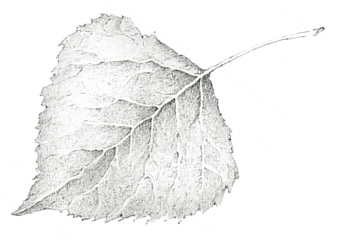
\includegraphics[width=0.6in,keepaspectratio,angle=190]{birch_by_Aj_Vimalo_3_CMYK.png}}}

\clearpage

\Section{Proti oceanu}

Ko se potoki, jezera in reke, ki tečejo proti oceanu, izlijejo vanj, so vsi enake modre barve in enakega slanega okusa.

Podobno je z ljudmi: ne glede na to, od kod prihajajo – ko dosežejo tok Dhamme, je to vedno ista Dhamma.

\Section{Podtalnica}

Buddha je Dhamma; Dhamma je Buddha. Dhamma, h kateri se je prebudil Buddha, je vedno tu. Ni izginila. Je kot podtalnica. Kdor koplje jašek za vodnjak dovolj globoko, bo slej ko prej naletel na vodo. S kopanjem jaška ne ustvari vode. Vse, kar naredi, je to, da vloži toliko svoje moči v kopanje jaška, da pride do vode, ki je že tam.

Torej, če smo količkaj bistri, bomo spoznali, da pravzaprav nismo daleč stran od Buddhe. Že zdaj mu sedimo nasproti. Kadar razumemo Dhammo, vidimo Buddho. Tisti, katerih namera je neprekinjena vadba Dhamme – ne glede na to, ali sedijo, stojijo ali hodijo –, so lahko prepričani, da bodo vedno slišali Buddhovo Dhammo.

\clearpage

\Section{Vse je tu}

Buddha je Dhamma; Dhamma je Buddha. Buddha ni vzel s seboj védenja, h kateremu se je prebudil. Pustil ga je prav tu. Vzemimo za primer šolske učitelje. Ne rodijo se kot učitelji. Preden postanejo učitelji, da lahko poučujejo v šolah in za to prejemajo plačilo, morajo najprej študirati. Čez čas začno pešati in slabeti. A s svojo smrtjo učitelji ne izumrejo. Lastnosti, zaradi katerih so postali učitelji, ostajajo tu. In prav tako je z Buddho. Plemenite resnice, ki so ga naredile za Buddho, so še vedno tu. Nikamor niso pobegnile.

\Section{Korenine}
Ljudje smo kot drevo s koreninami, z deblom in s krošnjo. Vsak list in vsaka veja sta odvisna od korenin, ki vsrkano hrano iz zemlje pošiljajo navzgor po drevesu.
Naše telo, besede, dejanja ter naša čutila za vid, sluh, vonj, okus in otip so kot veje, listi in deblo. Um je kot razvejane korenine, ki srkajo hrano in jo pošiljajo navzgor po deblu vejam in listom, da ti lahko cvetijo in obrodijo sadove.

\clearpage

\Section{Sloni, voli in vodni bivoli}
Pravilno urjenje uma je koristna dejavnost. To lahko vidimo celo pri vprežnih živalih, kot so sloni, voli in vodni bivoli. Preden jih uporabimo pri delu, jih moramo ustrezno uriti. Šele ko so dovolj izurjeni, lahko izkoristimo njihovo moč in jih uporabimo pri različnih opravilih. Vsi to že veste.

Dobro izurjen um je kar nekajkrat vrednejši od neurjenega. Poglejte Buddho in njegove plemenite učence. Iz ljudi, ki so se slepo vrteli v krogu, so se povzdignili v plemenite. Širše množice ljudi spoštujejo plemenite, saj so nam oni s svojimi dejanji pomagali v številnih smereh, ki si jih še predstavljati ne moremo. Vse to izvira iz dejstva, da so svoj um vpregli v pravilno urjenje.

Pravilno urjen um je koristen pri vsakem početju. Omogoča nam, da svoje delo opravljamo budno, previdno in pazljivo. Po njegovi zaslugi smo premišljeni, namesto da bi se prenaglili. Pravilno urjen um nam omogoča doživljanje sreče, ki ustreza našim življenjskim razmeram.

\clearpage

\Section{Izgubljena denarnica}

Tako je, kot če greste na sprehod in izgubite denarnico. Dokler ne ugotovite, da ste na poti izgubili denarnico, ste čisto zadovoljni – zadovoljni, ker pravzaprav še ne veste, zakaj pravzaprav doživljate to zadovoljstvo. Doživljate ga zaradi nezadovoljstva, ki bo nastopilo v trenutku spoznanja, da ste izgubili denarnico.

Podobno velja za naša slaba in dobra dejanja. Buddha nas je učil, da se moramo s temi stvarmi seznaniti. Če z njimi nismo seznanjeni, ne bomo imeli občutka za pravilno in napačno, za dobro in slabo.

\Section{Listje}

Ko sedimo v mirnem gozdu brez sapice vetra, vsi listi na drevju mirujejo. Ko zapiha veter, listi vztrepetajo.

Um je podoben listom. Ko se dotakne predmeta, zavibrira z naravo predmeta. Manj ko poznate Dhammo, bolj vaš um vibrira. Ko um doživlja ugodje, se izgubi v ugodju. Ko doživlja bolečino, se izgubi v bolečini. Takšen je njegov tok.

\clearpage

\Section{Kos ledu}

Če kos ledu postavite na sonce, lahko vidite njegovo taljenje, propadanje – enako se stara telo – zelo počasi, dan za dnem. Že po nekaj minutah, po nekaj urah se bo led stopil. To se imenuje \emph{khaya-vaya}: poslabšanje.

Že od samega začetka se vse sestavljene stvari razkrajajo in dosežejo svoj konec. Ko se rodimo, že vstopimo v ta proces. Ne moremo ga zaustaviti. Ko se rodimo, sprejmemo nase bolezen, staranje in smrt. Vse prevzamemo naenkrat.

Samo poglejte, kako se spreminja naše telo. Vsak del telesa se počasi stara. Lasje  in dlake postajajo redkejši, nohti so vse bolj krhki, koža je zgubana. Vse, čisto vse peša in se spreminja v skladu z naravnimi zakoni.

\clearpage

\Section{Voz in njegove sledi}

Krog ponovnih rojstev je kot kolo voza. Vol vleče voz. Če ga vleče brez ustavljanja, sledi kolesa brez prekinitev brišejo sledi vola. Kolesa voza niso dolga, so okrogla. Lahko bi rekli, da so dolga, a njihova dolžina je okrogla. Vidimo njihovo okroglost, ne vidimo pa njihove dolžine. Dokler vol vleče voz brez ustavljanja, se kolo voza vrti brez prekinitev.

Vol se ustavi. Utrujen je. Izpusti jarem. Vol gre svojo pot, voz gre svojo pot. Kolesa voza se počasi ustavijo. Če pustite voz dovolj dolgo stati na polju, bo razpadel in se spremenil v zemljo, vodo, veter in ogenj, povrnil se bo v travo in prst.

Enako je z ljudmi, ki še vedno ustvarjajo karmo: ne pridejo do konca. Ljudje, ki govorijo resnico, ne pridejo do konca. Ljudje z napačnimi pogledi ne pridejo do konca.

\clearpage

\Section{Otroci, izstrelki}

Pištola izstreli svoje otroke – izstrelke – navzven. Mi naše navznoter, v naše srce. Če so otroci dobri, smo ranjeni v srce. Če so otroci slabi, smo ranjeni v srce. Naši otroci zadevajo našo karmo. So dobri in so slabi, a oboji, dobri in slabi, so vsi naši otroci.

Samo poglejte nas, ko se nam rodijo otroci: bolj ko so slabega zdravja, raje jih imamo. Ko kateri od njih zboli za otroško paralizo in postane pohabljenec, imamo ravno tega najraje. Ko odhajamo od doma, naročimo najstarejšemu otroku, naj pazi na svojo mlajšo sestro, ker jo imamo tako radi. Še ko smo na smrtni postelji, rečemo najstarejšemu otroku: ">Pazi nanjo. Skrbi za mojega otroka."< Ker ni močna, jo še bolj ljubimo.

\clearpage

\Section{Kačji rep}

Mi, ljudje, nočemo trpljenja. Hočemo užitek. A užitek ni nič drugega kot prikrito trpljenje. Bolečina je očitno trpljenje. Če poenostavim, trpljenje in užitek sta kot kača. Njena glava je trpljenje; njen rep je užitek. Njena glava vsebuje strup. Strup se nahaja v njenih ustih. Če se približaš kačji glavi, te bo ugriznila. Če jo zagrabiš za rep, je to videti varno. A če jo držiš za rep, ne da bi jo izpustil, se kača lahko zasuka in te ugrizne, saj sta glava in rep dela iste kače.

Sreča in žalost izvirata od istih staršev: hrepenenja in iluzije. Čeprav ste dosegli stvari, ki jih visoko vrednotite, kot so materialni dosežki, položaj in pohvala, ste srečni, a v sebi še vedno nemirni in z neprijetnim občutkom. Srečni ste, a vaš um ni resnično miren, zaradi pritajenega suma, da lahko vse to izgubite. Skrbi vas, da bodo vaši dosežki izginili. Ta strah vas oddaljuje od miru. Zgodi se, da izgubite to, kar ste dosegli, in takrat resnično trpite. To pomeni, da je v stvareh, čeprav so prijetne, že prisotno trpljenje. A tega se ne zavedamo. To je enako, kot če zagrabimo kačo: čeprav jo zagrabimo za rep, če je ne izpustimo, se kača lahko zasuka in nas ugrizne.

Tako kot glava kače in njen rep, tako je z zlim in dobrim: tvorita krog, ki se neprestano obrača. Zato užitek in bolečina, dobro in slabo ne pomenijo tiste poti.

\clearpage

\Section{Kralj smrti}

Živimo kot kokoš, ki se ne zaveda, kaj se pravzaprav dogaja. Zjutraj odpelje svoje piščance na lov za hrano. Zvečer se vrne domov v kurnik. Naslednje jutro gre zopet ven in išče hrano. Lastnik vsak dan trosi riž, da ima kokoš kaj jesti, a ta ne ve, zakaj jo lastnik pravzaprav hrani. Kokoš in lastnik razmišljata različno.

Lastnik razmišlja: ">Le koliko tehta kokoš?"< Ko jo vzame v roke, da bi preveril njeno težo, kokoš, zatopljena v hranjenje, misli, da ji lastnik izraža naklonjenost.

Tudi mi ne vemo, kaj se dogaja: ne vemo, od kod prihajamo, koliko let življenja imamo še pred seboj, kam bomo šli, kdo nas bo peljal tja. Tega enostavno ne vemo.

Kralj smrti je kot lastnik kokoši. Ne vemo, kdaj nas bo dohitel, ker smo zatopljeni v zaznave vida, sluha, vonja, okusa, tipa in idej. Nimamo občutka, da se staramo. Nimamo občutka, da je nečesa dovolj.

\clearpage

\Section{Začetek je konec}

Ali veste, da smo ob rojstvu pravzaprav že mrtvi? Staranje in smrt sta isto. Poglejte drevo. En del drevesa, njegov začetek, so korenine; drugi del drevesa, njegov konec, je vrh. Če obstaja začetek, obstaja tudi konec. Če obstaja konec, obstaja tudi začetek. Če ni začetka, tudi ni konca. Če obstaja konec, mora obstajati tudi začetek. Konec se ne more zgoditi brez začetka; tega ni. Tako je to.

Pravzaprav je smešno. Ko nekdo umre, smo žalostni in vznemirjeni. Sedimo in jočemo, žalujemo – in počnemo vse, kar sodi zraven. To je iluzija. Veste, to je iluzija. Ko nekdo umre, jokamo. Tako je, odkar pomnimo. Pravzaprav – in oprostite, da se tako izrazim – se mi zdi, da bi bilo bolje, da jočemo, ko se nekdo rodi, in ne, ko umre. Mi smo to obrnili. Ko se rodi otrok, ljudje žarijo in se smejijo od sreče in veselja. A rojstvo je smrt. Smrt je rojstvo. Začetek je konec; konec je začetek.

\clearpage

\Section{Obarvana voda}

V običajnih razmerah je naše srce kot deževnica. Ta je čista, prozorna, prvinska in naravna. Če damo v vodo zeleno ali rumeno barvo, se bo obarvala zeleno ali rumeno.

Enako je z našim umom: ko se sreča s predmetom, ki mu je všeč, je srečen. Ko se sreča s predmetom, ki mu ni všeč, postane mračen in nemiren – ravno tako kot voda, ki se obarva zeleno, če spustimo vanjo zeleno, ali pa rumeno, če jo obarvamo z rumeno barvo. Kar naprej menja svojo barvo.

\Section{Sirota}

Če nihče ne nadzoruje našega uma, je ta kot otrok brez staršev – je kot sirota brez zaščitnika. Tako kot trpi oseba brez zaščitnika, se godi tudi umu. Če um ni urjen, če ni usmerjen v pravilno razmišljanje, zaide v številne težave.

\clearpage

\Section{Zakaj je težko}

Ko se pojavi trpljenje, moramo najprej spoznati, da gre za trpljenje in od kje pravzaprav izhaja ter kaj ga povzroča. Pa boste kaj videli? Če pogledamo na stvari iz pravega zornega kota, vidimo, da trpljenje ne obstaja. Na primer, ko sedimo tukaj, smo mirni. Pa pride trenutek, ko si zaželimo pljuvalnik in ga dvignemo. V tem trenutku so stvari drugačne od stanja, preden smo ga dvignili. Ko ga dvignemo, začutimo, kako nas njegova teža dodatno pritiska k tlom. Za to obstaja razlog. Kaj ne čutimo dodatne teže zaradi dvignjenega pljuvalnika? Če ga ne dvignemo, se ne zgodi nič. Če ga ne dvignemo, se počutimo običajno lahki. Torej, kaj je vzrok in kaj je posledica? Vse, kar moramo storiti, je to, da opazujemo, samo to. Ni se nam treba zapoditi v zapletena razglabljanja. Ko se nečesa oprimemo, je tu že vzrok za trpljenje. Ko spustimo stvari iz svojega prijema, izgine tudi trpljenje.

\clearpage

\Section{Injekcijska igla}

\ldots{}To je trpljenje. Običajno trpljenje je ena stvar; trpljenje, ki presega običajno trpljenje, pa je nekaj drugega. Običajno trpljenje muči naše telo. Muči ga, ko stojimo; muči ga, ko sedimo; muči ga, ko ležimo: to trpljenje je običajno trpljenje, normalno trpljenje našega telesa. Buddha je izkusil enake občutke. Občutil je enaka ugodja kot mi, pa tudi enake oblike trpljenja. A on je spoznal njihovo običajnost, naravnost. Običajne oblike ugodja in trpljenja je bil sposoben pripeljati do mirnosti, saj jih je razumel. Razumel je običajno trpljenje: bilo je, kakršno je pač bilo. Sploh ni bilo tako močno. Namesto potopitve v trpljenje se je postavil v položaj opazovalca, opazoval je trpljenje.

Podobno je, ko smo bolni in gremo k zdravniku po injekcijo. Injekcijska igla prodre skozi našo kožo v mišico. Malo boli, ampak to je običajna bolečina. Nič posebnega. Ne gre drugače. Trpljenje nad običajnim trpljenjem je \emph{upādāna} ali navezanost. To je tako, kot če bi injekcijsko iglo pred uporabo pomočili v strup. To ne boli kot običajno; to ni običajno trpljenje. To boli tako hudo, da nas lahko celo ubije.

\clearpage

\Section{Košček mesa, ki se zatakne med zobe}

Čutnim željam zelo težko pobegnemo. Čutne želje so podobne koščku mesa, ki se nam zatakne med zobe. O, kako to boli! Še preden zaključimo z obrokom, moramo seči po zobotrebcu, da se rešimo nadloge. Ko je zunaj, smo za trenutek olajšani pritiska in pravzaprav nimamo več želje po žvečenju mesa. Pa zopet žvečimo in se zopet zatakne. Vzamemo ga ven in si zopet oddahnemo. Tako je tudi s čutnimi željami: niso nič več kot košček mesa, ki se nam zatakne za zobe. Dokler se jih tako ali drugače ne znebimo, smo samo razburjeni in nemirni. Ne razumemo, kaj se pravzaprav dogaja. To je noro.

\Section{Drezanje v mravljišče rdečih mravelj}

Čutnost lahko primerjamo z drezanjem v mravljišče rdečih mravelj. Bolj ko drezamo, več rdečih mravelj nas napada, lezejo nam po obrazu, gredo nam v oči, oblegajo naša ušesa in oči. Ne opazimo, kaj počnemo. Dobro je, ko vemo in vidimo, kaj počnemo. Zapomnite si: če ne veste, kaj počnete, se ne boste nikoli rešili svojega početja.

\clearpage

\Section{Smrtna žeja}

Po dolgem potovanju človeka zelo zažeja. Sprašuje za vodo, vodnar pa mu odgovori: ">Lahko piješ to vodo, če želiš. Je prave barve, diši dobro, okusa je tudi dobrega, le želim, da veš, da je ta voda strupena. Lahko te ubije ali pa ti povzroči smrtne bolečine."< Žeja je premočna. Žejni popotnik ne posluša vodnarjevih besed.

Enako je s človekom po operaciji. Zapovedano mu je, da ne sme piti, a vseeno sprašuje za vodo.

Oseba, žejna čutnosti, je žejna vidnih užitkov, vonjav, zvokov, okusov, vsega, kar zastruplja.

Buddha nam govori, da so užitki preko vida, sluha, vonja, okusa, tipa in ideje strupeni. To so pasti. A ga ne poslušamo. Tako kot se za vsa opozorila ne zmeni žejni popotnik – pil bo ne glede na to, koliko težav in bolečin mu bo prineslo pitje strupene vode. Vse, kar želi, je le voda. Ne zmeni se, če bo po njenem zaužitju umrl ali pa se zvijal v smrtnih bolečinah. Takoj, ko v rokah začuti kozarec, ne more več zaustaviti svojega pitja. Človek, žejen čutnih užitkov, pije zaznave vida, sluha, vonja, okusa, tipa in idej. Ker so videti okusne, ne more nehati piti. Pil jih bo, dokler ne umre – ujet v dejanju, sredi čutnosti.

\clearpage

\Section{Ujeta žaba}

Živali, ujete v pasti in zanke, trpijo. Tesno so zvezane. Kar lahko naredijo, je le to, da čakajo na prihod lovca. Kot ptica, ki se ujame v zanko: zanka ji zadrgne vrat in ne glede na to, kako si ptica prizadeva uiti, zanka ne popusti. Ptica poskuša znova in znova, zaletava se naprej in nazaj, a ostaja ujeta. Vse, kar lahko naredi, je to, da počaka na lovca. Ko pa pride lovec, je konec. To je Māra. Ptice se bojijo lovca; vse živali se ga bojijo, ker se mu ne morejo izmuzniti.

Naše pasti so čutila vida, sluha, vonja, okusa, tipa in ideje. Zvezani smo z njimi. Ko smo navezani na vid, sluh, vonj, okus, tip in ideje, smo kot riba na trnku, ki čaka na ribiča. Ni važno, kako trpimo, ne moremo zbežati. Pravzaprav se nam godi slabše kot ujetim ribam. Bolj smo podobni ujetim žabam – saj ko žaba pogoltne trnek, se ta ustavi šele v njenem drobovju. Ribi pa se trnek zapiči v usta.

\clearpage

\Section{Kratka roka}

Buddhova učenja so neposredna, jasna in enostavna; kot taka pa so težka za tistega, ki z njihovo prakso šele pričenja, saj sposobnosti posameznikovega znanja ne morejo doseči Buddhovih učenj. Poglejmo primer luknje: ker ljudje ne morejo z roko doseči dna luknje, se pritožujejo, da je luknja globoka. Težko je v množici najti nekoga, ki bi uvidel, da dna ne more doseči zaradi prekratke roke.

Buddha nas je učil opuščanja kakršnega koli zla in škodljivosti. Ta del njegovega učenja radi preskočimo in se slepo lotimo ustvarjanja zaslug. Enako je, ko rečemo, da je luknja globoka.

Redki so tisti, ki priznajo, da je njihova roka kratka.

\Section{Trn}

Stvari so enostavno takšne, kot so. Ne povzročajo nam trpljenja. Kot trn: ali nam oster trn povzroča trpljenje? Ne. Trn je enostavno trn. Nikomur ne povzroča trpljenja. Če stopimo nanj, pa v trenutku trpimo.

Zakaj trpimo? Ker smo stopili nanj. Trpljenje izvira torej od nas.

\clearpage

\Section{Hov! hov! hov!}

Nekoč sem opazoval psa, ki sem mu dal jesti riž. Riža je bilo veliko, preveč, da bi ga pes pojedel vsega naenkrat. Ulegel se je poleg posode in budno čuval njeno vsebino. Bil je tako sit, da ni mogel več jesti, a kljub temu ni bil pripravljen deliti riža še s kom drugim. Kljub temu, da se mu je dremalo in da je bil zaspan, je ne glede na to, kako velik ali majhen pes se je približal njegovi posodi z rižem, vedno začel renčati. Če so se posodi približale kokoši, je začel lajati: Hov! Hov! Hov! Njegov želodec je bil tako poln, da bi lahko počil, a nikomur ni dovolil, da bi zaužil njegov preostanek. Bil je skopuški in sebičen.

Tudi ljudje so lahko takšni. Če ne poznajo Dhamme, če nimajo občutka za svoje dolžnosti do nadrejenih in podrejenih, če je njihov um preplavljen s pastmi pohlepa, jeze in iluzije, potem so skopuški in sebični, tudi če imajo dovolj premoženja. Ne vedo, kako to premoženje deliti. Težko jim je dati prostovoljni prispevek celo za revne otroke ali starce, ki nimajo hrane in so lačni. O tem sem pogosto učil in vedno znova me je pretresla podobnost ljudi z živalmi. Sploh nimajo človeških vrlin. Buddha jih je imenoval \emph{manussa-tiracchano}: ljudje-navadne-živali. Takšni so, ker nimajo vrlin dobre volje, sočutja, vživljajoče se radosti in ravnodušne mirnosti.

\clearpage

\Section{Pes na kupu neoluščenega riža}

\ldots{} Poglejmo, kaj se dogaja s psom, ki leži na kupu neoluščenega riža. Pes postane lačen in ko mu v želodcu prične kruliti, začne razmišljati: ">Le kje bi dobil hrano?"< Njegov želodec je lačen, zato skoči s kupa neoluščenega riža in se poda za iskanjem smeti.

Hrano ima pred smrčkom, v kupu riža, a je ne vidi. Ne vidi riža. Pes ne more jesti neoluščenega riža.

Znanje obstaja, a če ga ne spravimo v prakso, ga ne razumemo. Včasih smo tako neumni kot lačen pes na kupu neoluščenega riža. Res, prava škoda. Užiten riž je tam, a je skrit za lupinami – enako je z osvoboditvijo, ki je tu, a je skrita za našimi razglabljanji.

\clearpage

\Section{Garje}

Buddha je vprašal menihe: ">Menihi, ste videli šakala, ki je včeraj zvečer tekal tu naokrog? Ste ga videli? Ko je miroval, je trpel. Ko je tekal naokrog, je trpel. Ko je sedel, je trpel. Ko je ležal, je trpel. Ko se je zatekel v votlo deblo, je trpel. Ko se je zatekel v jamo, se je takoj počutil slabo. Trpel je, ker je mislil: 'Stati tukaj ni dobro. Sedeti ni dobro. Ležati ni dobro. To grmovje ni dobro. To votlo deblo ni dobro. Ta jama ni dobra.' Tako je nemirno tekal naokoli. V resnici pa je imel garje. Njegovo neugodje ni izviralo iz grma ali iz votlega debla ali iz jame, iz sedenja, stanja ali ležanja. Vir njegovega neugodja so bile garje ."<

Vi menihi ste prav takšni. Vaše neugodje izvira iz napačnega mišljenja. Držite se svojih idej, ki so vse strupene, in zaradi tega trpite. Ker ne sežete preko preprek vaših čutov, krivite druge. Ne veste, kaj se dogaja v vas. Ko ostanete tukaj v Wat Nong Pah Pongu, trpite. Greste v Ameriko in trpite tam. Greste v London in trpite. Greste v Wat Bung Wai in trpite. Obiščete vsak samostan in trpite. Kamorkoli greste, trpite. To trpljenje izvira iz napačnega mišljenja, ki vas še vedno obvladuje. Vaše mišljenje je napačno in v vaših srcih so ideje, ki so vse po vrsti strupene. Zato trpite, kamorkoli greste. Ste kot šakali.

Ko boste premagali vaše garje, boste mirni, kjerkoli boste: mirni boste zunaj, mirni boste v divjini. O tem velikokrat premišljujem in vam prenašam to učenje, saj je ta del Dhamme zelo koristen.

\enlargethispage{\baselineskip}

\clearpage

\Section{Ličinke}

Ko se v svojem srcu odpremo pravilnemu mišljenju, smo lahko mirni, kjerkoli že smo. Mirni nismo, ker se še vedno poslužujemo napačnega mišljenja in ker se držimo strupenih idej. Ob oklepanju tega smo podobni ličinkam. Umazanija je kot ličinkin dom; ličinkina hrana je umazana. Njena hrana ne ustreza hrani – a ustreza ličinki. Poskusite s palčko izbezati ličinko iz njenega govna in opazujte, kaj se dogaja. Ličinka se bo zvijala in zvijala, željna vrnitve v svoje govno. Šele tam se bo zopet počutila dobro.

Isto je z vami menihi in novici. Še vedno napačno razmišljate. Učitelji prihajajo in vas poučujejo, kako priti do pravilnega mišljenja, vendar vam to ne ugaja. Znova in znova se zatekate na svoj kup govna. Pravilno mišljenje vam ne diši, ker ste navajeni svojih kupov. Dokler ličinka ne spregleda umazanije svojega domovanja, ne more pobegniti od tam. In enako je z nami. Dokler ne spregledamo slabih strani našega mišljenja, jim ne moremo pobegniti. In te otežujejo našo prakso.

\clearpage

\Section{Reke}

Vse reke se vijejo v nižinski svet. Vijejo se navzdol v soglasju z naravo. Reka Ayutthaya, reka Muun – vzemite katerokoli reko hočete: vse se vijejo navzdol. Nobena ne teče navzgor. Tako je to.

Predstavljajte si človeka, ki na bregu reke opazuje rečni tok, kako nosi reko navzdol. Ob tem pa goji napačno mišljenje, saj bi hotel, da reka teče navzgor. S takšnim mišljenjem bo moral trpeti. Ne bo našel miru. Miru ne bo našel ne sede, ne stoje, ne hode in ne leže. Zakaj ne? Ker je njegovo mišljenje napačno.

\Section{Samotna pot}

Ne glede na to, kaj vse je v našem umu: če razlogi še niso dovolj dobri, stvari še ne bomo izpustili. Ali povedano drugače, vedno obstajata dve strani: ena je tu, druga je tam. Ljudje so navajeni hoditi vzdolž te strani ali pa vzdolž one. Skoraj nobenega ni, ki bi hodil po sredini. Ta pot je samotna pot. Ko je prisotna ljubezen, hodimo vzdolž ljubezni. Ko je prisotno sovraštvo, hodimo vzdolž sovraštva. Če poskušamo hoditi tako, da opuščamo ljubezen in sovraštvo, hodimo po samotni poti. Tej pa nismo voljni slediti.

\clearpage

\Section{Kokoš in raca}

Dva človeka vidita kokoš in raco. Prvi ima nenavadno željo: želi, da bi bila kokoš raca in raca kokoš. To enostavno ni možno, ni izvedljivo. Če ta človek ne bo spremenil svojega mišljenja, bo trpel. Drugi vidi kokoš kot kokoš in raco kot raco. Tu ni nikakršne težave. Ko so vaši pogledi pravi, ni trpljenja.

Enako velja tukaj. \emph{Anicca} – spremenljive stvari – poskušamo narediti stalne. Dokler so stvari nestalne, spremenljive, smo žalostni. V miru je lahko le tisti, ki vidi spreminjajočo se naravo stvari. V tem primeru ni nikakršne težave.

Že od rojstva naprej tečemo stran od resnice. Ne želimo in ne sprejmemo, da so stvari takšne, kot so; a drugačne sploh ne morejo biti. Stvari so pač takšne, spreminjajoče se. Ne morejo biti drugačne. To je ravno tako, kot bi se trudili doseči, da bi bila raca kokoš. Nikoli ne bo prišlo do tega. Ne more priti. Raca je raca. Kdorkoli si prizadeva stvari spremeniti v takšni smeri, bo moral trpeti. Če pa razmišljate takole: ">Aha, to je tako"<, potem ne izgubljate moči, temveč jo celo pridobite – ker ne glede na to, kako močno si prizadevate, nikoli ne boste dosegli stalnosti in trajnosti vašega telesa.

\clearpage

\Section{Neslana sol}

Nekoč me je obiskal menih, ki je zase trdil, da je meditant, in me vprašal, ali bi lahko živel pri meni. Zanimala ga je naša praksa in pojasnil sem mu: ">Če živiš z menoj, ne moreš posedovati ne denarja ne drugih stvari. Sledim poti Vinaye."<

Rekel je, da prakticira nenavezanost.

Odvrnil sem: ">Ne vem, kaj misliš s tem."<

Zato je vprašal: ">Ali lahko bivam tukaj, če uporabljam denar, ne da bi bil navezan nanj?"<

Na to sem mu odgovoril: ">Seveda. Če lahko ješ sol in ne čutiš slanosti, potem lahko ostaneš tukaj. Če pa le trdiš, da si nenavezan, ker se ti ne da upoštevati teh nadležnih pravil, potem boš težko ostal tukaj. Če pa lahko ješ sol, ne da bi čutil njeno slanost, ti bom verjel. Ali lahko resnično poješ vedro soli, ne da bi čutil njeno slanost? Ta nenavezanost, o kateri govoriš, ni nekaj, o čemer bi samo govoril ali o njej ugibal. Če govoriš tako, ne moreš živeti z menoj."<

In menih je odšel.

\clearpage

\Section{Prenašanje skale}

Dejanski pomen opuščanja: to je tako, kot če bi nosili težko skalo. Ko jo nosimo, čutimo, da nas vleče navzdol, vendar ne vemo, kaj naj z njo storimo, zato jo nosimo naprej. Ko nam nekdo reče, naj jo odvržemo, si mislimo: ">Hm? Če jo odvržem, mi ne bo ostalo nič."< Zato jo še naprej prenašamo. Nismo je pripravljeni odvreči.

Četudi nam nekdo reče: ">Daj no, odvrzi jo. Bolje bo zate, koristilo ti bo,"< skale še vedno nismo pripravljeni odvreči, ker se bojimo, da nam ne bo nič ostalo. Tako jo nosimo, vse dokler nismo tako izčrpani in utrujeni, da je ne moremo več nositi. Takrat jo spustimo.

Šele ko jo spustimo, razumemo, kaj pomeni opustiti. Počutimo se lahkotni. V sebi lahko začutimo, kakšno težo smo občutili med prenašanjem skale. Ko smo jo nosili, se sploh nismo zavedali, kako koristno je opuščanje.

\clearpage

\Section{Iver}

Buddha nas uči, naj ubežimo s pomočjo pravilnega razumevanja. To je tako, kot da imamo v stopalu drobceno iver ali trn. Ko hodimo, nas včasih boli in včasih ne. Če udarimo ob panj, nas zaboli. Čutimo celo stopalo, vendar ne čutimo iveri in zato vse skupaj pustimo. Čez nekaj časa se udarimo v prst na nogi in zapičena iver nas spet začne boleti. In vse se vedno znova ponavlja. Zakaj? Ker je iver ali trn še vedno v našem stopalu. Še vedno ni zunaj. Bolečina se vrača. Ko boli, tipamo za iverjo, vendar je ne najdemo, zato vse skupaj spet pustimo. Potem znova boli in znova jo poskušamo poiskati in zatipati. Vse se kar naprej ponavlja. Ko se bolečina pojavi, moramo ugotoviti, kaj je. Ni nam treba pustiti, da le izzveni. Ko nas stopalo boli, si mislimo: ">Oh, ta presneti trn je še vedno tu."<

Ko se pojavi bolečina, se z njo pojavi tudi želja, da bi trn izvlekli. Če ga ne bomo izvlekli, se bo bolečina vračala, vračala in znova vračala. Naša želja, da bi izvlekli trn, obstaja ves čas. Na koncu bo le prišel dan, ko se bomo ne glede na vse odločili, da ga moramo zaradi bolečine izvleči.

Naša odločenost, da vložimo energijo v prakso, mora biti taka. Kjerkoli obstaja motnja, kjerkoli obstaja neudobje, moramo stvari takoj raziskati, takoj razrešiti težavo – rešiti težavo s trnom tako, da ga takoj izvlečemo.

\clearpage

\Section{Ribarjenje na slepo}

\ldots{} Vse dokler ne vidite nevarnosti stvari v tolikšni meri, da bi jih opustili, dotlej ne vidite nagrad, ki bi jih s tem dobili, in vaše delo ne bo doseglo namena. Tako je, kot bi se le igrali s stvarmi, kot bi le z nohti praskali po njih. Če jasno vidite njihove slabosti, vidite nagrade, ki jih prinaša opuščanje – ah!

To je tako, kot če bi s košaro lovili ribe. Vztrajate in čakate, vse dokler ne začutite nečesa v košari. Slišite hrup, ki ga povzroča nekaj, kar se zaletava ob stene košare. Mislite si, da je riba, in zato sežete v košaro in tipate po njej, toda kar zatipate, ni riba. Nekaj drugega je, kar živi v vodi. Z očmi ne morete ugotoviti, kaj je. Del vas si misli, da je mogoče jegulja, drugi del pa si misli, da bi lahko bila kača. Bilo bi vam žal, če bi bila jegulja, vi pa bi jo izpustili. Toda, če je kača in vi jo držite v roki, vas lahko ugrizne. Razumete? V dvomih ste, ker stvari niso jasne. Vaša želja je tako močna, da kar naprej držite, ker bi lahko bila jegulja. Ko jo izvlečete iz vode in vidite vzorec na njenem vratu, jo takoj izpustite. Nikogar ni, ki bi vam lahko rekel: ">To je kača! Spusti! Spusti!"< Nihče vam tega ne reče. Um reče sam sebi – celo jasneje, kot če bi vam to rekel nekdo drug. Zakaj je tako? Ker vidite nevarnost: kača lahko ugrizne. Kdo mora reči umu? Če ga urite, dokler ne vé na ta način, se ne bo oklepal.

\clearpage

\Section{Pljuvalnik}

O \emph{anatti}: preprosto povedano, \emph{anatta} pomeni 'ne-jaz'. Vendar je to odvisno od tega, da obstaja občutek jaza; odvisno je od tega, da obstaja občutenje \emph{atte}. Zato obstaja \emph{anattā}. Zato je tudi \emph{anattā} pravilna. Če ni \emph{atte}, se tudi \emph{anattā} ne pojavi. Na primer: v hiši nimate pljuvalnika, zato vas nič v zvezi s pljuvalnikom ne skrbi. Najsi se razbije ali poči ali pa ga ukradejo tatovi, nič od tega ne obremenjuje vašega srca – saj ni razloga, ni okoliščin. Zakaj je tako? Ker v vaši hiši ni pljuvalnika.

Če pa je v vaši hiši pljuvalnik, je to občutek jaza, ki se pojavlja. Ko se pljuvalnik razbije, vas to zadeva. Ko se izgubi, vas to prizadene – ker ima pljuvalnik zdaj lastnika. To se imenuje \emph{atta}. To je njeno stanje. Stanje \emph{anatte} pa pomeni, da v hiši ni pljuvalnika in zato ni stanja uma, ki bi moralo skrbeti zanj in ga varovati. Ni strahu, da ga bodo ukradli tatovi. Teh stanj ni več.

To imenujemo stanje stvari.\footnote{sabhāva-dhamma} Obstajajo stanja in razlogi zanje, vendar samo obstajajo, to je vse.

\clearpage

\enlargethispage{10cm}

\Section{Olupki in lupine}

Povedal vam bom preprosto primerjavo. Recimo, da ste na tržnici kupili banano ali kokos in sadež zdaj nosite s seboj.

Nekdo vas vpraša: ">Zakaj si kupil banano?"<

">Kupil sem jo, da bi jo pojedel."<

">Toda, ali moraš pojesti tudi olupek?"<

">Ne."<

">Ne verjamem ti. Če ga nisi hotel pojesti, zakaj ga potem nosiš s seboj?"<

Ali, denimo, da ste kupili kokosov oreh:

">Zakaj nosiš kokosov oreh?"<

">Domov ga nesem, da bom pripravil kari."<

">In vanj boš dal tudi lupino?"<

">Ne."<

">Zakaj pa jo potem prenašaš s seboj?"<

Torej, kako boste odgovorili na to vprašanje?

Skozi željo. Če ni želje, potem se ne more pojaviti iznajdljivost, razsodnost.

Tako je tudi, ko se trudimo v meditaciji. Čeprav to počnemo z opuščanjem, je tako kot z banano ali kokosovim orehom. Zakaj nosite olupek ali lupino? Ker še ni prišel čas, da bi ga odvrgli. Še vedno varuje notranje meso. Ni še pričel čas, da bi ga odvrgli, zato ga za zdaj še nosite.

Enako je z našo prakso: domneve in njihovo opuščanje morajo biti združeni, ravno tako kot sta združena kokosova lupina in njegovo meso, saj zato ju nosimo skupaj. Če nas obtožijo, da jemo koksovo lupino, kaj potem? Mi vemo, kaj počnemo.

\clearpage

\Section{Računanje}

Dhamma je kot računanje. Obstajajo množenje, deljenje, seštevanje in odštevanje. Če lahko tako razmišljamo, bomo inteligentni. Poznamo pravi čas in kraj za uporabo teh funkcij. Odštevamo, ko moramo odštevati, množimo, ko moramo množiti, delimo, ko moramo deliti, in seštevamo, ko moramo seštevati. Če bi ves čas množili, bi se srce strlo pod bremeni. Z drugimi besedami, takrat nimamo občutka za to, kdaj je dovolj. Ko nimamo občutka, kdaj je dovolj, pomeni, da ni občutka, da se staramo. 

Vsakdo, ki ima občutek staranja, ima tudi občutek za dovolj. Ko je razvit ta občutek, se lahko pojavijo besede: ">Dobro, to je dovolj."< Če ni občutka za dovolj, se tisti 'dobro, to je dovolj' ne more pojaviti, saj si še naprej želimo jemati. Nikoli nismo ničesar odvrgli, ničesar opustili, ničesar odložili. Vedno jemljemo. Če lahko rečemo 'dobro, to je dovolj', potem smo umirjeni, sproščeni. To je dovolj.

\clearpage

\Section{Razbit kozarec}

Lahko rečete: ">Ne razbij mojega kozarca,"< vendar ne morete preprečiti, da se ne bi razbilo nekaj, kar se lahko razbije. Če se ne razbije zdaj, se bo razbilo kasneje. Če ga ne boste razbili vi, ga bo nekdo drug. Če ga ne bo nekdo drug, ga bodo kure! Buddha pravi, naj to sprejmemo. On je prodrl tako globoko, da je videl kozarec že razbit. Sporoča nam, da je kozarec, ki ni razbit, že razbit. Kadarkoli vzamete kozarec in pijete iz njega ter ga odložite, nam pravi, da je kozarec že razbit. Razumete? Buddha je to razumel tako. V celem kozarcu je videl razbitega. Ko se prenehajo pogoji zanj, se razbije. Razvijte to naravnanost. Kozarec uporabljate, pazite nanj, potem pa vam nekega dne zdrsne iz roke: ">Pok!"< Nič hudega. Zakaj ni nič hudega? Ker ste ga videli razbitega, še preden je bil razbit. Razumete?

Običajno ljudje rečejo: ">Tako dobro sem skrbel za ta kozarec. Nikoli nisem dopustil, da bi se razbil."< Kasneje ga razbije pes in vi ga zato sovražite. Če ga razbije vaš otrok, sovražite tudi njega. Sovražite kogarkoli, ki ga razbije – saj ste se tako zajezili, da ni pretoka. Zgradili ste jez brez možnosti izlitja. Jez zato lahko le poči, ni res? Ko zgradite jez, morate zagotoviti tudi izlitje. Ko voda doseže neko raven, lahko varno odteče stran. Ko je jez poln do roba, lahko voda varno odteče. Imeti morate tako izlitje. To, da vidi nestalnost, je Buddhovo izlitje. Ko stvari vidite tako, ste lahko mirni. To je praksa Dhamme.

\clearpage

\Section{Obiranje manga}

Če želimo obrati mango, ki raste na višini petih metrov, ne moremo uporabiti desetmetrske palice, da bi ga dobili, saj je palica predolga. Tudi dvometrske palice ne moremo uporabiti, saj je prekratka.

Nikar ne mislite, da ima oseba z doktoratom láhko delo s prakticiranjem Dhamme, ker toliko vé. Ne mislite tega. Ljudje z diplomo so včasih predolgi.

\Section{Sol}

Če delate dobro, da bi se rešili trpljenja, morate istočasno delati dobro in razvijati veščine v umu. Če teh veščin ne razvijete, ne bo pravilne  razsodnosti. Dobro samo po sebi je kot surovo meso ali surova riba. Če jo zgolj pustite tako, kot je, se bo pokvarila. Če pa jo posolite ali postavite v hladilnik, bo zdržala dolgo časa.

\clearpage

\Section{Narobe obrnjen bazen}

Ko enkrat opustimo zla dejanja, potem tudi, kadar le tu in tam naredimo nekaj dobrega, še vedno ostaja upanje, da se bo naša popolnost razvila v celoti. Tako kot bazen, ki ga postavimo na prostem: tudi če le rahlo rosi, obstaja možnost, da se bo napolnil.

Če pa delamo dobro, ne da bi opustili zlo, je tako, kot bi bazen postavili narobe. Ko dežuje, še vedno pada na dno bazena, vendar od zunaj in ne od znotraj. Ni mogoče, da bi voda napolnila bazen.

\Section{Bazen, ki pušča}

Če počnemo zlo in poskušamo razpoko v našem delovanju zamašiti z dobrimi deli, je to enako, kot če bi na dnu vrča želeli zamašiti razpoko, hkrati pa bi na vrhu vanj zlivali vodo. Dno vrča, dno bazena ni v dobrem stanju. Četudi vanj zlivamo vodo, na dnu še vedno pušča in bazen ostane prazen. Tudi če cel dan vanj prilivamo vodo, še vedno pušča in na koncu v njem ne bo vode. To nam ne koristi tako, kot bi si želeli.

\clearpage

\Section{Voda v vrču}

Ko v našem srcu ni nikakršne oblike zla, izginejo vse naše težave. Pojavi se občutek prisebnosti, saj dobro skrbimo zase. Um postane poln vrlin. Ko se umiri, se osredotoči. Ko je umirjen, se začne razcvetati v razsodnosti. Vemo, kako ustvariti jasen in svetleč um. Pustimo, da gre, kar je zlo. Odstavimo vse, kar je narobe. Meditiramo in stvarem pustimo, da odidejo, ali pa jih odstavimo.

Podobno je z vodo v vrču. Iz vrča zajamemo vodo in jo zavržemo. Z zajemalko zajamemo drugič in vodo zopet zavržemo – neprestano zajemamo vodo in jo mečemo stran. Vode v vrču bo slej ko prej zmanjkalo. Um, ki se poda v prakso, je tudi tak.

Toda če stvari ne vidimo takih, potem je tako, kot bi vodo v vrč vlivali in jo potem zajemali, dodajali in jemali. Dobra dela, zla dela, dobra dela, zla dela; napačno, pravilno, napačno, pravilno; dobro, slabo, dobro, slabo: za trenutek v miru in potem spet trpimo.

\clearpage

\Section{Kalup}

Vi učitelji ste kalup za oblikovanje ljudi, zato bi se morali obrniti v smeri Dhamme in jo prakticirati. Obnašajte se tako, da boste zgled drugim. Ste kot kalup za amulete s podobo Buddhe. Ste kdaj kakšnega videli? Le en kalup: dobro ga izrezljajo, izrezljajo obraz, obrvi, brado, tako da nič ne manjka in ni nepravilno, tako da so amuleti Buddhe, ki jih z njim naredijo, resnično čudoviti – vse zaradi tega dobrega kalupa.

Enako je z učitelji. Učitelji so kalup za svoje učence in ljudi na splošno. Tudi vi morate biti brezhibni glede osebnostnih lastnosti dobrega učitelja. Vedno se morate vesti v skladu s svojo etično disciplino in vzorcem voditelja in vodnika. Opustite vse oblike omamljanja in neprimernega vedenja. Poskusite obuditi visoka merila moralnosti. Biti morate dober zgled otrokom.

\clearpage

\Section{Ovijalke}

Otroci so kot ovijalke. Kjerkoli ovijalka vzbrsti, mora poiskati drevo, po katerem bo plezala. Kaj mislite, po katerem drevesu bo plezala, če je eno drevo oddaljeno petnajst centimetrov in drugo deset metrov? Ovila se bo okoli najbližjega drevesa. Najverjetneje se ne bo ovila okoli drevesa deset metrov stran, ker je ta predaleč.

Na enak način so učitelji najbližji ljudje svojim učencem. Učitelji so ljudje, ki jih bodo učenci najverjetneje imeli za vzor. Zato je bistvenega pomena, da se znate vi, učitelji, dobro vesti in da poznate oliko – glede tega, kaj bi morali početi in kaj opustiti –, da otroci to vidijo. Nikar jih ne učite samo z besedami. Vaša drža, vaša hoja, vaše sedenje – vsak vaš premik, vsaka vaša beseda – naj otroke učijo. Sledili bodo vašemu zgledu, saj otroci hitro posnemajo stvari. Hitreje kot odrasli.

\clearpage

\Section{Čaša umazane vode}

Veliko ljudi, ki pride sem, ima visok položaj v družbi in oblikovana stališča: o sebi, o meditiranju, nekateri imajo diplome, nekateri so učitelji ali državni uradniki. Njihovi možgani so polni stališč o vseh možnih stvareh. So preveč pametni, da bi poslušali druge. To je kot voda v čaši. Če je čaša polna umazane vode, je ne moremo uporabiti za nič. Šele ko iz nje izlijemo vodo, jo lahko znova uporabimo. Iz svojega uma morate umakniti stališča, šele potem se boste lahko učili.

Naša praksa seže prek bistrosti in neumnosti. Če mislite: ">Pameten sem. Bogat sem. Pomemben sem. Vsa Buddhova učenja razumem,"< ne boste nikoli videli resnice \emph{anatte} ali ne-jaza. Ničesar drugega ne boste imeli razen jaza – jaz in moje. Toda Buddhovo učenje pomeni opuščanje jaza. Praznino. Osvoboditev od trpljenja. Popolno razpustitev. To je \emph{nibbāna}.

\clearpage

\Section{Vaš notranji snemalnik}

Učenje, ki sem vam ga podal danes: če je ob poslušanju te Dhamme vaš um postal miren in prazen, to zadošča. Ni si vam treba ničesar zapomniti. Nekateri med vami morda tega ne verjamete. Če umirite svoj um in dovolite, da vse, kar slišite, zdrsne mimo, vendar še vedno motrite, ste kot snemalnik. Kadarkoli je um tako odprt, tako vključen, je vse tukaj. Ne bojte se, da ne bo ničesar. Vsakič, ko odprete svoj snemalnik, ga vključite, vse je tukaj.

Zunanji snemalniki lahko zatajijo. Ko jih kupite, lahko zatajijo. Toda vaš notranji snemalnik, ko gredo stvari neposredno v srce: ">Oh, ta je še kako dober!"< Notranji snemalnik je vedno tu in zanj ne potrebujete baterij.

\clearpage

\Section{Baloni}

V Buddhovih časih so nekateri med sedenjem in poslušanjem Dhamme prodrli v njeno najvišjo stopnjo. Bili so hitri. Kot balon: zrak v balonu ima moč, da se potisne navzven. Ko balon predrete z iglo, prične zrak takoj z vso močjo uhajati.

Podobno je tudi s tem. Ko slišite Dhammo v skladu z vašimi nagnjenji, preobrne vaša stališča, od tega k onemu, in prodrete lahko v resnično Dhammo.

\Section{V primerjavi z volom}

Vol vleče natovorjen voz – bliže ko sta večer in sončni zahod, hitreje hodi, saj si želi čim prej priti na cilj. Vol pogreša svoj dom.

Pri ljudeh pa je tako: starejši ko smo, bolj smo bolni, bliže smo smrti in umiranju – ravno to pa je čas, ko je treba prakticirati. Starost in bolezen ne smeta biti razlog, da ne prakticirate – če ne, boste slabši kot voli.

\clearpage

\Section{Srce je svoj lastni učitelj}

Vsi tukaj smo enaki. Ne razlikujemo se drug od drugega. Zdaj nimamo učitelja – če naj bi se prebudili v Dhammo, mora srce učiti samo sebe. Če srce ne uči samega sebe, potem je popolnoma vseeno, koliko nas učijo drugi, saj srce ne bo poslušalo, ne bo razumelo. Srce samo mora biti učitelj.

Ni nam lahko videti samih sebe. Težko je. Zatorej razmislite malce o tem. Vsi smo že storili kaj slabega. Zdaj, ko smo stari, bi morali s tem prenehati. Naj nam bo lažje. Naj bo slabega manj. Dejansko ne gre za nič drugega. To je vse, kar je. Obrnite svoj um proti vrlinam.

\Section{Voda in olje}

Voda se razlikuje od olja, ravno tako kot se bistri ljudje razlikujejo od neumnih. Buddha je živel s pogledi, zvoki, vonji, okusi, dotiki in idejami, vendar je bil \emph{arahant}, zato je stvari videl preprosto takšne, kot so, to je vse. Opuščal je, vse odkar je videl, da je srce samo srce, to je vse. Misli so le misli. To je vse. Ni jih mešal, združeval.

Če lahko mislite tako, če lahko čutite tako, lahko stvari ohranjate ločene. Misli in občutja so na eni strani, srce je na drugi – tako kot sta v steklenici ločena voda in olje.

\clearpage

\Section{Domnevni menihi, resnični menihi}

Ko vas posvetijo v Buddhova učenja, si domišljate, da ste menih. Vendar v resnici še niste. Menih ste toliko, kot je menih vaše telo: obrita glava, rumena oblačila. Menih ste na ravni domneve.

Enako je, kadar rezbarijo les, oblikujejo cement ali vlivajo bron, da bi dobili Buddho na ravni predpostavljanja. To ni resnični Buddha.

Menihi, ki so še vedno menihi na ravni domneve, so z drugimi besedami tisti, ki še poznajo pohlepa, jeze in zablod srca. Te stvari nas zadržujejo v stanju začetka in rojstva. Razlog, da ne dosežemo miru, leži v pohlepu, jezi in zablodah. Če iz srca preženete pohlep, jezo in zablode, boste dosegli čistost. Dosegli boste resnično meništvo. To pomeni, da boste v srcu menih.

\clearpage

\Section{Najprej delo, potem plačilo}

Nekateri ljudje pridejo prakticirat, da bi dosegli užitek in nič drugega. Toda, od kod pride užitek? Kaj je njegov namen? Vse oblike užitka morajo slediti in izhajati iz bolečine. Šele potem lahko pride do užitka. Najsi počnemo karkoli – najprej moramo delati, šele potem dobimo plačilo, s katerim lahko kaj kupimo. Mar ni tako? Najprej moramo delati na polju, če hočemo dobiti riž. Vse mora najprej skozi bolečino in trpljenje.

\vspace{-\baselineskip}
\Section{Izdelovanje miz in stolov}

Dobro je, če je naš um čist in umirjen, vendar tudi težko. Začeti je treba z zunanjim – telesom in besedami – šele potem lahko napredujemo. Pot, ki vodi h čistosti, k stanju motrenja, je pot, ki lahko izmije pohlep, jezo in zablode. Vaditi morate vzdržnost in samoobvladovanje, zato je to težko. A kaj potem, če je težko?

Podobno je, kot če bi hoteli iz kosa lesa narediti mizo ali stol. Težko je, pa kaj potem? Les mora skozi ta proces. Preden lahko postane miza ali stol, mora skozi grobe in težke faze.

Enako velja za nas. Postati moramo vešči tam, kjer še nismo, občudovanja vredni, kjer še nismo, in usposobljeni tam, kjer še nismo.

\clearpage

\Section{Stonoga}

Ko se nas veliko zbere in so naša stališča pravilna in usklajena, je lahko prakticirati. Ko smo se pripravljeni na enak način ukloniti in opustiti ponos, se vsi zberemo na ravni Buddhe, Dhamme in Sanghe. Ne morete reči, da številčnost menihov moti vašo prakso. To je tako kot pri stonogi, ki ima veliko nog. Ko jo pogledate, bi si mislili, da se bo toliko nog zagotovo zapletlo. Vendar lepo hodi. Hodi naprej in nazaj in se nikoli ne zmede. Ima svoj ritem in svoj red.

Enako je z Buddhovimi učenji: če prakticirate Buddhovo učenje, je lahko. Drugače rečeno – prakticirate pravilno, natančno in brez kompromisov, prakticirate, da bi se osvobodili trpljenja. Tudi če nas je na stotine, tisoče, kolikor že, nič hudega. Vsi se lahko pridružimo istemu toku.

\clearpage

\Section{Pometanje}

Dnevna opravila nam dajejo moč. Kjerkoli v samostanu jih lahko opravljate – najsi gre za vašo kolibo ali kolibo koga drugega; če je umazana ali razmetana, jo lahko počistite ali pospravite. Tega vam ni treba početi zaradi nekoga drugega. Na nikogar vam ni treba delati vtisa. To naredite zaradi svoje prakse. Ko pometamo svoje kolibe, je tako, kot bi pometali umazanijo iz svojih src, saj smo ljudje, ki prakticiramo. Želim si, da bi vsak od nas imel tako naravnanost v svojem srcu. Potem nam ne bo treba prositi za usklajenost ali sodelovanje, saj bosta že prisotna.

\vspace{-2\baselineskip}
\Section{Saditi poprovec}

Buddha, naš učitelj, je dejal, da je od stvari samih odvisno, kako se odvijajo. Četudi vztrajamo in se trudimo pri praksi, ne moremo vplivati na to, kako hitro ali počasi bo šlo. Tako je, kot ko sadimo poprovec. Rastlina sama ve, kaj počne. Če si želimo, da bi hitro rasla, je to utvara. Če si želimo, da bi rasla počasi, je tudi to utvara. Le če jo dejansko posadimo, bomo dobili sadež, ki si ga želimo.

Ko sadimo poprovec, moramo izkopati jamo, zaliti rastlino, jo pognojiti, se znebiti škodljivcev. To je vse. To je odvisno od nas, od našega prepričanja. Ali bo rastlina pognala ali ne, pa je odvisno od nje. Ni odvisno od nas. Rastline ne moremo raztegovati, da bi rasla.

\clearpage

\Section{Pot v samostan}

Vrline, koncentracija in pravilno razumevanje: te stvari je Buddha imenoval pot. Pot ni religija in ni tisto, kar je Buddha dejansko hotel, temveč je le orodje, da prispemo.

To je tako, kot ko se odpravite iz Bangkoka do Wat Nong Pah Ponga. Niste si želeli, da bi sem prišla cesta. Želeli ste si le priti v samostan. Vendar ste za to potrebovali cesto. Cesta, ki pride sem, ni samostan. Je le cesta do samostana. Slediti morate cesti, da pridete do samostana.

Vrline, koncentracija in pravilno razumevanje so cesta do miru – in mir je to, kar si v resnici želimo doseči.

\vspace{-\baselineskip}
\Section{Zdravilo}

\ldots{} To je kot zdravnik, ki da bolniku z vročino stekleničko zdravil. Na steklenički je nalepka, ki pojasnjuje, katere bolezni lahko zdravilo pozdravi. Zdravilo, ki zdravi bolezni, pa je v steklenički. Če bolnik zapravlja svoj čas za branje nalepke – tudi če jo bere stokrat, tisočkrat, bo na koncu morda umrl in od zdravila ne bo imel nobene koristi. Godrnjal bo in se pritoževal, da je njegov zdravnik nesposoben, da zdravilo ne more pozdraviti bolezni, za katere trdi, da jih lahko – četudi sploh ni odprl stekleničke, da bi iz nje vzel zdravilo.

\clearpage

\Section{Drgnjenje paličic za netenje ognja}

Praksa je kot človek, ki drgne paličice za netenje ognja. Slišal je ljudi reči: ">Vzameš dva koščka bambusa, ju drgneš drugega ob drugega in dobiš ogenj."< Zatorej vzame dva koščka bambusa in ju drgne. Toda v srcu je nestrpen. Čeprav ju drgne le kratek čas, že želi, da bi se ogenj zanetil. Njegovo srce priganja, da bi se ogenj hitro zanetil, toda ognja kar noče biti. Počasi postaja len, zato se ustavi, da bi počival. Potem spet kratek čas poskuša in se zopet ustavi, da bi počival. Kolikor je sploh bilo toplote, se razgubi, saj ni povezana.

Če bo še naprej tako ravnal, se zaustavljal, kadarkoli bo utrujen (čeprav samo to, da si utrujen, sploh ni tako slabo), se bo vmešala še njegova lenoba in mu ne bo uspelo. Odločil se bo, da ognja ni, da si ga pravzaprav sploh ne želi, in se bo vdal. Prenehal. Paličic ne bo več drgnil. In potem bo govoril: ">Ognja ni. Tako ga ne zanetiš. Ognja enostavno ni. – Sem že poskusil."<

\vspace{-2.5\baselineskip}
\Section{Ključ meditacije}
\vspace{-0.5\baselineskip}

Praksa je kot ključ, ključ meditacije. Ni pomembno, kakšna je ključavnica, saj imamo ključ zanjo že v rokah. Ne skrbi nas, kako tesna je ključavnica, saj vsakič, ko obrnemo ključ, dosežemo svoj namen. Če ključavnica nima ključa, ne moremo doseči svojega namena. Tega, kar je zaklenjeno, ne moremo dobiti.

\clearpage

\Section{Vroče in hladno}

\ldots{} Podobno je s tem: kjerkoli gori ogenj, tam tudi ugasne. Kjerkoli je vroče, tam se ohladi. Tako je tudi \emph{nibbāna} tam, kjer je \emph{samsāra}, in kakor je v naravi stvari, je \emph{samsāra }tam, kjer je \emph{nibbāna}. Ravno tako, kot sta vroče in hladno na istem mestu: hladno je tam, kjer je vroče. Ko postane vroče, hladno izgine. Ko pa hladno izgine, postane vroče\ldots{}

\Section{Proti toku}

Prakticirati pomeni iti proti toku: proti tokovom v srcu, proti toku slabosti. Karkoli gre proti toku, mora biti močno. Veslati po reki navzgor je težko. Vzpostavljanje dobrote in vrlin je precej težko, ker smo ljudje polni slabosti, in tega si ne želimo. S tem se ne želimo obremenjevati. Ne želimo si graditi vztrajnosti. Večinoma si želimo, da bi stvari potekale v skladu z našimi razpoloženji. Tako kot voda, ki teče v skladu s svojo strugo. Lahko je pustiti, da stvari tečejo s tokom, vendar to ni praksa. Pri praksi se moramo upirati. Upirati se moramo slabostim, upirati lastnemu srcu, prisiliti svoje srce in povečati moč svoje vztrajnosti. To pomeni, da gremo pri praksi proti toku.

\clearpage

\Section{Mačka}

Slabosti so kot mačka. Če jo nahranite, kadarkoli se ji zahoče, se bo vračala vse pogosteje. A nekega dne vas bo opraskala, če je ne boste nahranili. Zato vam je ni treba hraniti. Mijavkala bo in mijavkala, toda če ji dva, tri dni ne daste hrane, ne bo več prihajala.

Podobno je s slabostmi. Če jih ne hranite, vas ne bodo obremenjevale. Vaš um se lahko potem umiri.

\Section{Sladkorni trs}

Ste kdaj jedli sladkorni trs? Veste, kako je, če ga grizljate od vrha proti korenini? Bolj ko se približujete korenini, slajši je – do točke, ko ga ostane le še pet centimetrov, vi pa ga ne želite odvreči. Škoda vam ga je. Mravlje si ga želijo, vendar jim ga ne boste prepustili.

Naj bo tudi vaša praksa taka. Vadite Dhammo kot nekdo, ki jé sladkorni trs.

\clearpage

\Section{Ograja}

Prakso začnemo tako, da vzpostavimo moč svoje vztrajnosti in potem razmišljamo. Razmišljamo o svojih dejanjih, o čemerkoli, kar počnemo. O tem, kaj dosegamo. Karkoli se pojavi, nas Buddha pripravi na vse. Iz katerekoli smeri se pojavijo stvari, vse poznamo. Če poznamo vse, vidimo vse, kar pride. Pravilno poznamo. Napačno poznamo. Srečno poznamo. Zadovoljno poznamo. Poznamo vse.

Toda, ko razmišljamo, naš um še ni vsepovsod, ne pozna vsega. Poznamo le eno plat, drugo puščamo odprto. To je tako, kot bi okrog polja ali hiše postavljali ograjo, a je ne bi postavili vsenaokrog. Če postavimo ograjo samo na eni strani, se bodo tatovi prikradli na drugi strani, na strani, kjer ograje ni. Zakaj? Nismo zaprli vrat. Naša ograja še ni popolna. Zato je razumljivo, da se bodo prikradli skozi luknjo. Zato spet razmišljamo in brez postanka dodajamo ograjo ter tako preprečujemo vdor.

Postavitev ograje pomeni, da vzpostavimo pozornost in smo vselej čuječni. Če to počnemo, Dhamma ne bo izginila. Točno tukaj bo. Dobro in slabo, Dhamma, ki bi jo morali videti in poznati, se bo pojavila natanko tu.

\clearpage

\Section{V obliki kroga}

Ne mislite, da morate sedeti, če želite meditirati, da morate hoditi naprej in nazaj, če želite meditirati. Ne mislite tako. Meditacija je preprosto stvar prakse. Najsi pridigate, sedite tukaj in poslušate ali odhajate od tu – obdržite prakso v srcu. Bodite pozorni na to, kaj je prav in kaj ne.

Ne mislite, da zadošča, če sledite asketski praksi med trimesečnim umikom v deževnem obdobju in jo opustite, ko se umik konča. To ni dovolj. Stvari se ne uravnotežijo tako. To bi bilo tako, kot če bi izsekovali polje. Izsekujemo in izsekujemo ter se zaustavimo, ko smo utrujeni. Odložimo orodje in se vrnemo čez mesec ali dva. Zdaj je plevel višji od štorov. Preveč in pretežko bi bilo zdaj očistiti območje, ki smo ga že očistili.

Ajahn Mun je nekoč dejal, da bi morala naša praksa imeti obliko kroga, kajti krog se nikjer ne konča, in naj se praksa nadaljuje, nadaljuje brez prekinitve. Poslušal sem ga in pomislil: ">Kaj naj storim, ko se bo končalo to učenje, ko bom nehal poslušati?"<

Odgovor je v tem: naj vaša čuječnost postane \emph{akāliko} – brezčasna. Poskrbite za to, da bo um védel in videl, kaj je pravilno in kaj ni. Vsak trenutek.

\clearpage

\Section{Požari in poplave}

Buddha je učil, da sta um in telo takšna, kot sta, in da bosta še naprej ostala takšna. Ne bosta drugačna. Z drugimi besedami: najprej se pojavita, se postarata, razbolita in potem umreta. Babica, takšna je prava resnica, ki jo izkušaš zdaj. To je plemenita resnica. Zatorej jo opazuj z razsodnostjo, da jo boš videla. To je vse.

Tudi če tvojo hišo uniči požar, tudi če jo uničijo poplave, bo to prizadelo le tvojo hišo, tvoj dom. Če gori, naj ne zgori tvoje srce. Če voda poplavlja, naj ne poplavi tvojega srca. Naj poplavi le hišo. Naj pogori le hiša – to je nekaj, kar je zunaj, kar ni tvoje telo. Tvoje srce naj vse to opusti, kajti zdaj je primeren čas. Čas je za opustitev.

\Section{Spustiti kozarec}

Prakticirajte z opuščanjem. Ne oklepajte se ničesar. Če pa že nekaj držite, ne držite močno. Razumete, kaj pomeni 'ne držati'? Recimo, ta kozarec tukaj: primemo ga, da bi ga dvignili in pogledali. Ko o njem vemo vse, ga položimo nazaj. To pomeni 'ne držati'. Z drugimi besedami: držimo, a ne močno. Držite, da bi pogledali in védeli, in potem odložite. Mirni ste, sproščeni. Enako je z opuščanjem.

\clearpage

\Section{Zastrupljena banana}

V samostan sem prišel pri devetih letih, ko sem bil posvečen v meniha pripravnika. Poskušal sem prakticirati, vendar takrat nisem kaj dosti razumel. Razumevati sem začel šele, ko sem bil posvečen v meniha. Oho! Zdaj sem v vsem videl strah. Opazoval sem čutnost, v kateri živijo ljudje, in namesto da bi se mi zdela nekaj zabavnega kot njim, sem jo doživljal kot trpljenje. Kot čokoladno bananico. Ko jo jemo, je okusna in sladka. Njena sladkost nam je domača. Če pa vemo, da jo je nekdo zastrupil, nam ni več mar za to, da je sladka, saj se zavedamo, da bomo umrli, če jo pojemo, kajne? Tako sem torej vedno dojemal stvari. Ko naj bi zagriznil v nekaj mamljivega, sem se zavedel dodanega strupa. In tako sem se vse bolj oddaljeval od čutnosti in ostal menih vsa ta leta. Kadar razumeš, te ne premami več, da bi poskusil takšno jed.

\vspace{-\baselineskip}
\Section{Študij ali bitka}

Nekateri menihi so učenjaki – preučujejo tekste, ves čas študirajo. Pravim jim, naj poskusijo s prakso. To zvesto ravnanje po knjigah: ko študiraš, si resda v skladu z besedili, a ko greš v bitko, se moraš oddaljiti od njih. Če se bojuješ samo po navodilih iz knjig, ne boš kos sovražniku. Kadar gre zares, moraš delovati onstran knjig.

\clearpage

\Section{Roka}

Tisti, ki preučujejo tekste, in oni, ki prakticirajo Dhammo, pogosto ne razumejo drug drugega. Preučevalci tekstov imajo navado reči: ">Menihi, ki ne delajo drugega kot meditirajo, govorijo preprosto v skladu s svojimi pogledi."< To pravijo, ne da bi imeli za to kakršenkoli dokaz.

Obstaja prispodoba, v kateri sta obe plati medalje eno in isto in ki nam pomaga bolje razumeti reči. Pomislite na dlan in hrbtno stran svoje roke. Če iztegnete roko naravnost predse, se zdi, kot da je dlan izginila. A v resnici ni nikamor izginila, je le skrita pogledu. Prav tako izgine hrbtna stran vaše roke, če obrnete dlan navzgor. A tudi ta ni izginila, je le na spodnji strani.

Tega se morate spomniti, ko začnete meditirati. Če mislite, da se je vaše meditiranje razvodenelo, prenehajte preučevati Dhammo in stavite vse na doseganje rezultatov. Ne glede na to, koliko ste se posvetili preučevanju Dhamme, je ne boste razumeli, ker vaše védenje ni v skladu z resnico. Šele ko razumete pravo naravo Dhamme, začnete opuščati stvari. To je pripravljenost odpovedati se navezanostim, ko se ne oklepate ničesar več. Če pa že, je tega oklepanja postopoma vse manj in manj.

V tem je razlika med študijem in meditacijsko prakso.

\clearpage

\Section{Nož}

Urjenje telesa in urjenje uma z namenom, da bi ju okrepili, sta istovrstno početje, le metodi sta različni. Pri urjenju telesa razgibavaš njegove različne dele, ko pa uriš um, ga ustaviš in počivaš, tako kot pri koncentraciji. Poskusi pripraviti svoj um do tega, da opusti vse. Naj se ustavi samo ob enem predmetu. Tako se bo okrepil. Nastalo bo pravilno razumevanje. To je tako kot pri nabrušenem nožu. Če ga uporabljaš za rezanje kamnov, opeke, trave, ne da bi pazil, kaj režeš z njim, nož izgubi ostrino.

\Section{Zapisane besede}

Ustavi se. Pospravi svoje intelektualno znanje. Ne pusti mu do besede. Te vrste znanja tu ne potrebuješ. Tu gre za znanje druge vrste. Ko stvari dejansko nastajajo, gre za nekaj drugega.

Podobno je, kot če bi napisal besedo 'pohlep'. Ko se pohlep pojavi v srcu, to ni isto kot zapisana beseda. Tako je tudi, če si jezen: če napišeš 'jeza' na tablo, je to ena stvar. To so črke. Ko pa se jeza pojavi v tvojem srcu, se vse odvija prehitro, da bi karkoli prebral. V srcu se pojavi kar naenkrat. To je pomembno. Zelo pomembno.

\clearpage

\Section{Padec z drevesa}

\ldots{} Enako je z odvisnim sonastajanjem. ">Nevednost je pogoj za tvorbo. Tvorba je pogoj za zavest. Zavest je pogoj za ime in obliko."< To smo preučili in si zapomnili, in res je, tako je Buddha razdelil stvari, da bi jih učenci lažje doumeli. A ko vsaka od njih dejansko nastane, se to zgodi prehitro, da bi jih lahko razločevali.

Tako kot pri padcu z drevesa – bum! – na tla. Ne vemo, mimo katerih vej smo padali. V trenutku, ko se v umu pojavi predmet, ki mu je všeč, se takoj pojavi misel 'dobro'. Um ne razloči med vmesnimi koraki, ki so pripeljali do tega. Ti si sledijo tako, kot je zapisano v knjigah, ampak sežejo tudi onkraj napisanega. Dogajanje ni opisano: ">Tu je nevednost. Tu je tvorba. Tu je zavest. Tu sta ime in oblika."< Ni znakov, iz katerih bi prebrali posamezne korake. Tako kot pri padcu z drevesa. Buddha zelo podrobno govori o trenutkih v mišljenju, jaz pa uporabljam primerjavo s padcem z drevesa. Ko zgrmiš z drevesa – bum! –, ne meriš, koliko metrov in centimetrov si padel. Veš samo to, da si priletel na tla in da te boli.

\clearpage

\Section{Učenje pisanja}

Poskrbi za to, da boš prakticiral vsak dan, vsak dan. Nadaljuj tudi, če se počutiš lenega. Nadaljuj, kadar se počutiš discipliniranega. Prakticiraj Dhammo podnevi in ponoči. Nadaljuj, kadar je um miren. Nadaljuj tudi, kadar ni miren. Tako kot v otroštvu, ko si se učil pisati. Sprva črke niso bile lepe. Bile so prevelike ali premajhne. Pisal si kot otrok. Sčasoma pa so postajale vse lepše, ker si vadil.

\Section{Otrok in odrasel}

Koncentracija in pravilno razumevanje morata nastopati skupaj. V prvi fazi se bo um umiril z metodami koncentracije. Lahko bo ostal miren samo, če sediš z zaprtimi očmi. To je umirjenost. Zanesti se moraš na koncentracijo, ki bo omogočila nastanek pravilnega razumevanja ali na koncu uvida. Potem pa bo um ostal enako miren, če sediš z zaprtimi očmi ali se sprehajaš po mestnem vrvežu.

To je tako: nekoč si bil otrok. Zdaj si odrasel. Otrok in odrasel sta ista oseba. Prav tako bi lahko rekel, da sta umirjenost in uvid dve ločeni stvari. Ali hrana in izločki: lahko rečeš, da so ista stvar, a gledano z drugega zornega kota lahko tudi rečeš, da so različni.

\clearpage

\Section{Palica}

Meditacija je kot palica. Na enem koncu palice je uvid, na drugem koncu pa umirjenost. Če dvigneš palico, ali se bo z njo dvignil samo en konec ali se bosta dvignila oba? Seveda oba. Karkoli je uvid, karkoli je umirjenost, vse je um.

\Section{Slikanje slike}

Uspeh pri prakticiranju je povezan s pravilnim razumevanjem: meditacijo uvida, kjer sta združena pravilno razumevanje in um. Nekaterim ljudem ni treba veliko, da se jim to dvoje spoji samo od sebe. Ljudem, ki znajo opazovati, ni treba dosti. Koncentracija je nekaj podobnega kot biti umetnik. Že ko nekaj pogledaš, razumeš. Z razumevanjem to ostane v tvojem srcu. Iz tega, kar je v tvojem srcu, lahko naslikaš sliko. Ni ti treba sedeti pred predmetom in ga slikati po videnem. Človek, ki ne razume, pa mora imeti predmet vedno pred seboj in ga skicirati toliko časa, dokler mu ne prodre v srce. Tistemu, ki zna opazovati, to ni potrebno. Pogleda in razume. Slikaš lahko neposredno iz svojega razumevanja. Tako je to.

\clearpage

\Section{Hrana, ki ti je všeč}

Predmet meditacije za razvoj miru, ki ne ustreza našemu značaju, ne bo privedel do miru oziroma pomiritve strahu. Predmet, ki je v skladu z našim značajem, pa je pogosto v naših mislih. Tega ponavadi niti ne opazimo, a če bi želeli imeti kakšno korist od njega, bi morali biti pozornejši na to. To je tako kot pri ponudbi različnih jedi na pladnju. Če poskusiš vsako od njih, boš najbolje vedel, katera ti je všeč in katera ne. Za tiste, ki ti prijajo, boš rekel, da so okusnejše od drugih. Tu govorim o hrani. A to lahko primerjaš s svojo meditacijo. Katerikoli predmet, ki je v skladu s tvojim značajem, ti bo ustrezal.

\clearpage

\Section{Lov na kuščarja}

Osredotočenje uma na predmet pomeni, da spoznaš svoj um in da spoznaš svoj predmet. Tako kot pri lovu na kuščarja. Kuščar se skriva v votlini termitnjaka, ki ima šest izhodov. Lovci pet izhodov zaprejo in pustijo odprtega samo enega, skozi katerega naj bi prišel kuščar na plano. Potem sedijo pred tem izhodom in ga opazujejo. Ko kuščar prileze skozenj, ga lahko ujamejo.

Na enak način osredotoči svoj um. Zapri oči, zatisni si ušesa in nos, utišaj jezik in pozabi na telo, samo tvoj um naj bo odprt. Z drugimi besedami, uri se v obvladovanju svojih čutov in se osredotoči samo na um.

Meditacija je kot lov na kuščarja. Um osredotoči na dihanje, s pozornostjo in pazljivostjo zbudi zavest. Pri kateremkoli početju bodi čuječen. Občutek, ki v takem trenutku nastane v umu, je, da se zavedaš tega, kar počneš. Ta občutek je tisti, ki te dela zavestnega.

\clearpage

\Section{Voda kaplja, voda teče}

Začni s poglabljanjem v lastni um. Pri tem vedno pazi, da upoštevaš pet vodil. Če narediš napako, se ustavi in začni vse od začetka. Morda te bo spet zapeljalo vstran in boš naredil novo napako. Ko to ugotoviš, se vrni na začetek in začni znova, vselej in vsakokrat.

Tvoja pozornost bo vse bolj zgoščena; kot voda, ki jo nalivamo iz kotlička. Če kotliček rahlo nagnemo, bo voda iz njega kapljala: plink \ldots{} plink \ldots{} plink. Curek je prekinjen, s premori. Če kotliček nagnemo malce bolj, si kaplje hitreje sledijo: plink-plink-plink. Če pa kotliček še bolj nagnemo, posamezne kaplje izginejo in voda teče v neprekinjenem curku. Ni več posameznih kapljic, čeprav niso te nikamor izginile. Le tako hitro sledijo druga drugi, da so se spremenile v en sam tok vode. Postale so tako goste, da so onkraj pogostosti. Vse se zlijejo v en curek.

\clearpage

\Section{Paša vodnih bivolov}

\ldots{} Prav tako je pri meditaciji. Kadar motrimo naš um, kadar zavest opazuje svoj lastni um, bo tistemu, kar nadzoruje um, uspelo ubežati Mārovim pastem.

Tako je kot pri paši vodnega bivola: na eni strani imamo riževe rastlinice, na drugi bivola, na tretji pa njegovega lastnika.

Bivol ima najraje riževe sadike. So njegova priljubljena hrana. Um je kot bivol. Njegovi predmeti so kot riževe sadike. Zavest je kot bivolov lastnik. Ko pasemo bivola, mu moramo slediti, da se ne bi spravil na riževe poganjke. Pustimo ga, da se prosto pase, a ga pri tem poskušamo nadzorovati. Čim se približa riževemu polju, začnemo kričati nanj. Ko nas zasliši, se ustavi. Vendar ne smemo biti prehitro zadovoljni sami s sabo. Vsekakor ne smemo zadremati sredi belega dne. Če to storimo, riževih poganjkov zagotovo prav hitro ne bo več.

\clearpage

\enlargethispage{2\baselineskip}

\Section{Kadar moramo premlatiti bivola}

Um je kot bivol. Njegovi predmeti so kot riževe rastline. Zavest je kot lastnik bivola. Kako pasemo vodnega bivola? Pustiti mu moramo, da se prosto pase, a hkrati moramo bdeti nad njim. Če se približa riževim poganjkom, zakričimo. Ko nas zasliši, se umakne. A pri tem ne smemo biti prehitro zadovoljni sami s sabo. Če je bivol trmast in naše kričanje ne zaleže, moramo vzeti debelo palico in ga pošteno namlatiti z njo.

Kaj mislite, kam bo šel potem?

\vspace{-\baselineskip}
\Section{Vzgoja otroka}

\ldots{} Pri tej praksi naj bi sedeli. To je sedeča meditacija. Potem opazujete. Pojavila se bodo dobra in slaba razpoloženja, pomešana med seboj, v skladu z njihovo običajno naravo. Ne hvalite ali kaznujte svojega uma kar tako. Počnite to z občutkom za čas in prostor. Ko nastopi primeren trenutek za hvalo, ga malce pohvalite – ravno prav, ne preveč, da ga ne razvadite. To je tako kot pri vzgoji otroka. Včasih ga morate našeškati. Vzemite šibo in ga nekajkrat mahnite po riti. Temu se preprosto ne morete izogniti. Z drugimi besedami, otroke je včasih treba kaznovati.

Ne smete pa jih kaznovati ves čas. Če jih ves čas kaznujete, bodo zašli na stranpota. Če pa nenehno skrbite za njihovo ugodje in jih nagrajujete, ne bodo sposobni priti nikamor.

\clearpage

\enlargethispage{2\baselineskip}

\Section{Pravilna oblika}

Običajni način sedeče meditacije in osredotočanja pozornosti je, da sedimo s prekrižanimi nogami, desna noga je nad levo, prav tako je desna roka nad levo. Sedimo vzravnano. Nekateri pravijo, da lahko meditiramo med hojo ali sede; torej lahko to morda počnemo tudi kleče? Gotovo – a vi ste šele začetniki. Ko se učite pisanja, morate najprej vaditi vsako črko posebej, z vsemi njenimi posebnostmi. Ko že obvladate črke in pišete samo zase, lahko tudi čečkate, če hočete. Nič ni narobe s tem. Ampak najprej se morate naučiti pravilne oblike.

\vspace{-2\baselineskip}
\Section{Sejanje riža}

Sedi in opazuj svoj vdih in izdih. Bodi sproščen, naj ti bo udobno, ampak ne dovoli, da te kaj zapelje vstran. Če se ti to zgodi, se ustavi. Opazuj, kam je zaneslo tvoj um in zakaj ne sledi več dihanju. Pojdi za njim in ga pripelji nazaj. Naj sledi tvojemu dihu in enkrat te dni ti bo uspelo najti nekaj dobrega. Ampak vztrajaj pri tem, kar počneš. To počni tako, kot da od tega nič ne pričakuješ, kot da se nič ne bo zgodilo, ne veš, kdo sploh to počne – samo vztrajaj. To je tako, kot bi jemal riž iz košare in ga sejal po zemlji. Videti je, kot bi ga metal stran. Stresaš ga po zemlji, kot da te to sploh ne zanima. Ampak iz njega zrastejo poganjki in sadike. Rastlinice posadiš na riževem polju in na koncu si nagrajen z riževimi posladki. Tako je to.

\clearpage

\enlargethispage{2\baselineskip}

\Section{Učenje otroka}

Včasih dihanje ni pravilno. Dih je predolg ali prekratek in te spravlja v obup. To je zato, ker svojo pozornost premočno usmerjaš nanj, preveč pritiskaš na svoj um. Kot bi učil otroka sedeti. Če ga vsakič udariš, bo zaradi tega postal kaj pametnejši? Preveč ga nadziraš. Enako je pri dihanju. Razmisli: ko se sprehodiš od hiše do sadovnjaka ali greš od doma v službo, zakaj te dihanje takrat ne obremenjuje? Zato, ker ga ne nadzoruješ. Pustiš ga pri miru, da poteka v skladu s svojim naravnim ritmom. Deli telesa te bolijo, ker je tvoja pozornost pretirano osredotočena nanje.

\vspace{-2\baselineskip}
\Section{Nagajiv otrok}

To je tako, kot kadar nagajiv otrok uganja norčije in nas tako dolgo jezi, da moramo zakričati nanj in ga našeškati. Razumeti moramo: gre preprosto za to, da je takšna njegova narava. Ko to dojamemo, ga lahko pustimo, da se naprej igra. Občutek nadležnosti in razdraženosti bo izginil sam od sebe, ker smo pripravljeni sprejeti, da je to v njegovi naravi. Na takšen način se spremenijo naši občutki glede nečesa.

Ko sprejmemo naravo stvari, jim lahko pustimo, da izginejo, ne ukvarjamo se več z njimi. Takrat je naš um miren in sproščen. To pomeni, da smo pravilno razumeli. Imamo pravilen pogled. Tako je konec težav, ki jih moramo rešiti.

\clearpage

\Section{Slovo od sorodnika}

Opazuj dihanje. Osredotoči se nanj. Usmeri vanj svojo pozornost. Z drugimi besedami, um naj se zaveda dihanja v tem trenutku. Ni se ti treba zavedati veliko reči. Bodi pozoren samo na vajo uma, ki bo vse bolj pretanjen, postopoma, nenehno, dokler ne postane občutek diha čisto izostren in je um izredno buden.

Vse bolečine, ki se pojavijo v telesu, se bodo postopoma umirile. Na koncu boš opazoval dihanje kot sorodnika, ki te je prišel obiskat. Ko odhaja, ga pospremiš do avtobusne postaje ali pomola. Pospremiš ga do avtobusa, do ladje. Ko vžgejo motor, se avtobus ali ladja odpelje, ti pa stojiš na postaji, pomolu in opazuješ, kako se oddaljuje. Sorodnik je odpotoval, ti se vrneš domov.

Enako je pri opazovanju dihanja. Kadar je dihanje težko, vemo. Kadar je umirjeno, vemo. Ko postaja vse bolj enakomerno, še naprej opazujemo, sledimo dihu, smo pozorni na to, kaj se dogaja z umom, dosežemo, da je vse budnejši, pustimo dihanju, da postaja vse bolj pretanjeno. Nazadnje je že tako rahlo, da ni več ne vdiha ne izdiha. Ostane samo občutek budnosti.

\clearpage

\Section{Čuječnost}

Če minutko nisi pazljiv, si to minuto nerazsoden. Če pozornost popusti za dve minuti, si dve minuti nerazsoden. Če popusti za pol dneva, si nerazsoden pol dneva. Tako je to.

Pozornost pomeni, da svoj um usmerimo. Kadar nekaj storimo ali rečemo, ne smemo pozabiti na čuječnost. Ko nekaj počnemo, smo pozorni na svoje početje. To je tako, kot bi imeli v hiši razprodajo. Na očeh imamo stvari, ki jih prodajamo, morebitne kupce in tatove, ki nam bi radi ukradli naše stvari. Če smo nenehno pozorni na vse to troje, bomo vedeli, po kaj je kdo prišel. Kadar imamo v rokah to orožje – smo torej ves čas na preži –, bodo tatovi to opazili in si ne bodo upali krasti.

Enako je s predmetom, na katerega je osredotočen um. Če smo pozorni in čuječni, se nam ne more nič zgoditi. Vemo: dober predmet nas ne bo vedno razveseljeval. To ni nekaj gotovega. Vsak trenutek lahko izgine. Zakaj bi se ga torej oklepali? ">Tega ne maram"<: tudi to ni nekaj nespremenljivega. Če je torej tako, so predmeti preprosto brezpredmetni; to je vse. Če se tega učimo, ostajamo pozorni, nenehno skrbimo zase: podnevi, ponoči, kadarkoli.

\clearpage

\Section{Obiski}

Naj bo tvoj um zavesten in buden. Nenehno ga opazuj. Če pride kdo na obisk, ga odslovi. Sedež je samo eden, ni prostora za obiskovalce. Poskusi sedeti na mestu in sprejemati obiske cel dan. To je mišljeno z besedo \emph{buddho}. Ne premakni se z mesta. Vzdržuj pozornost, da lahko ves čas nadzoruje um. Ko sediš tu, na svojem mestu, bodo vsi obiskovalci, ki prihajajo k tebi že od nekdaj – vse od rojstva, ko si bil še drobceno bitje –, prišli sem, k tebi, ki si sam in v stanju 'budnega'.

Goste pa, obiskovalce, ki se pojavljajo in si izmišljajo vse mogoče –, pusti, da so, kakršni so, vsak v skladu s svojo naravo. Um jih spremlja, gre z njimi – to se imenuje \emph{cetasika}. Karkoli je, kamorkoli gre, koga briga? Seznani se samo z obiskovalci, ki bi radi ostali. Imaš samo en sedež, kamor jih lahko posadiš, zato je lahko na njem v nekem trenutku samo en obiskovalec. Drugi se nimajo kam usesti. No, ko pridejo prvič in se hočejo pogovarjati s tabo, se ne bodo uspeli usesti. Ko pridejo naslednjič, kadarkoli to bo, bodo vedno naleteli na nekoga, ki sedi tu in se ne premakne nikamor. Kolikokrat bodo še prišli, če so prišli samo zaradi klepeta s tabo? Vse jih boš spoznal, vse tiste, ki prihajajo že od nekdaj, od takrat, ko si se prvič začel zavedati stvari. Vsi bodo prišli na obisk.

\clearpage

\Section{Kokoš v kletki}

Ko se združita pozornost in um, ki opazuje, nastane poseben občutek. Če je um pripravljen, da se umiri, bo ujet na mirnem kraju, kot kokoš, ki smo jo dali v kletko. Ne more iz nje, ampak lahko se sprehaja po njej. Njeno stopicanje sem ter tja ne povzroča težav, saj to počne v kletki. Občutki uma, kadar uporabljamo pozornost za vzdrževanje njegovega miru, občutki tistega mirnega kraja niso nekaj, kar bi nas lahko vznemirilo. Z drugimi besedami, kadar čuti, kadar razmišlja, naj se počuti znotraj miru. Tako ne bo težav.

\Section{Živeti s kobro}

Zapomnite si nekaj: vsi predmeti uma, ne glede na to, ali gre za stvari, ki jih imamo radi ali ne, so kot strupene kobre. Če vas napadejo in pičijo, lahko umrete. Predmeti so kot kobre z močnim strupom. Predmeti, ki jih imamo radi, so zelo strupeni. Predmeti, ki jih ne maramo, so prav tako zelo strupeni. Zaradi njih um ne more biti svoboden. Zapeljejo ga stran od načel Buddhove Dhamme.

\clearpage

\Section{Pustimo kobro na miru}

Predmeti in razpoloženja uma so kot kobre z močnim strupom. Če kobri nič ne prekriža poti, bo v skladu s svojo naravo spolzela mimo nas. Čeprav je strupena, tega ne bo pokazala. Če se ji ne približamo, nas ne bo ogrožala. Spolzela bo mimo, v skladu s svojo naravo. Šla bo svojo pot.

Če smo pametni, bomo pustili vse na miru. Dobre stvari, slabe stvari, stvari, ki jih maramo – pustimo jih na miru, tako kot strupeno kobro. Pustimo ji, da gre svojo poti. Spolzi mimo nas, četudi je strupena.

\Section{Mangi na tleh}

Izkoristite svoje mirovanje za razmislek o videnem, slišanem, vonjih, okusih, dotikih in mislih ne glede na to, ali so dobri ali slabi, veseli ali žalostni. Tako je, kot če nekdo spleza na mangovec in ga trese, da sadeži popadajo na tla. Mi smo pod drevesom in pobiramo sadeže. Ne poberemo gnilih, ampak samo tiste, ki so užitni. Nič energije nismo porabili, saj nismo sami plezali na drevo. Samo pobiramo sadeže, ki so padli z drevesa.

\clearpage

\Section{Žgalna peč}

Poskusite v sebi, zase, te stvari videti jasno: to se imenuje \emph{paccattam}. Katerikoli zunanji predmet se pojavi v vašem umu, je vedno in brez prestanka vaša osebna izkušnja, \emph{paccattam}. Povedano s preprostimi besedami, tako je, kot bi žgali oglje ali opeko. Ali ste že kdaj videli peč za žganje oglja ali opeke? Meter okrog ustja peči zakurijo ogenj, peč pa povleče dim in ogenj vase. Tako si to predstavljajte. Na ta način vam bo jasneje. To je primerjava. Če zgradite peč za žganje oglja ali opeke pravilno, v skladu z navodili, zakurite ogenj meter ali poldrugi meter okrog ustja peči. Ko se dim začne dvigati, ga vsega povleče v peč in nič ga ne ostane zunaj. Toplota gre v peč, se tam razbuhti in ne uhaja ven. Vsa toplota se posrka v peč in tam zelo hitro žge, kar je v njej. Tako je to.

Tako je tudi z občutki človeka, ki prakticira meditacijo: zazdi se, da je vse usmerjeno v pravilno videnje. Oko vidi oblike, uho sliši zvoke, nos zaznava vonjave, jezik okuša okuse – vsi pa se usmerijo v pravilno videnje. Tako nastane povezava, ki vedno znova vodi v pravilno razumevanje.

\clearpage

\Section{Pajek}

Dober primer sem našel pri opazovanju pajkov. Pajek gradi pajčevino v obliki mreže. Tke pajčevino in jo širi, tako da jo pripne na različne oporne točke. Nekoč sem tako sedel in opazoval pajka. Razobesil je svojo pajčevino kot filmski zaslon in ko je končal, se je mirno zvil v klobčič, ravno na sredini mreže. Ni plezal naokrog. Če se je muha ali kakšna druga žuželka zaletela v njegovo mrežo, se je pajčevina zatresla. Čim se je zatresla, je pajek prihitel iz svojega središča in ujel žuželko za svojo hrano. Ko se je najedel, se je spet zvil sredi svoje pajčevine kot poprej. Ni bilo važno, kakšna žuželka se je ujela v njegovo mrežo, čebela, karkoli: takoj ko se je pajčevina zatresla, je pajek pohitel na lov. Potem se je spet umaknil in vsakič umiril na sredini svoje mreže, kjer ga nihče ni mogel videti.

Ob opazovanju takšnega pajkovega vedenja sem nekaj spoznal. Sfere šestih čutil so oko, uho, nos, jezik, telo in um. Um je v sredini, oko, uho, nos, jezik in telo pa so razprostrti okrog njega kot mreža. Predmeti čutov so kot žuželke. Takoj, ko pogled doseže oko, zvok uho, vonj nos, okus jezik ali občutek dotika telo, je um tisti, ki ve. Stvari zavibrirajo naravnost do uma. To je dovolj, da nastane razumevanje.

Lahko živimo tako, da se zvijemo vase, kot se pajek zvije v klobčič sredi svoje mreže. Ni nam treba nikamor. Ko se žuželka ujame v mrežo in ta prenese tresljaj do srca, se takoj, ko se zavemo, poženemo iz sredine in ujamemo žuželko. Nato pa se vrnemo na svoje prvotno mesto.

Po opazovanju pajka lahko naučeno uporabite za svoj um. Gre za enak pojav. Če um zazna nestalnost, nezadovoljivost in nesebstvo, se na široko razpre. Nič več si ne lasti sreče ali trpljenja, saj tako šele jasno vidi. Dojame. Karkoli počnete, ste sproščeni. Ničesar več si ne želite. Vaša meditacija lahko napreduje.

\AddToShipoutPicture*{\put(\LenToUnit{1.5in},\LenToUnit{2in}){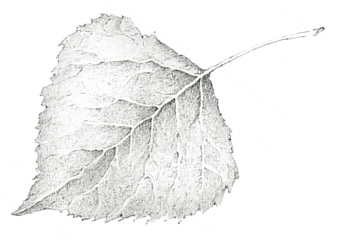
\includegraphics[width=0.6in,keepaspectratio,angle=-60]{birch_by_Aj_Vimalo_3_CMYK.png}}}

\clearpage

\Section{Divje kokoši}

Povedal vam bom enostaven primer, kako je z divjimi kokošmi. Vsi vemo, kako se obnašajo. Ni živali na svetu, ki bi bila tako preplašena pred človekom. Ko sem prvič prišel v ta gozd, sem jih privadil nase. Opazoval sem jih in se od njih marsičesa naučil.

Sprva si je samo ena upala priti mimo mene, ko sem prakticiral meditacijo v hoji. Ko se mi je približala, sem gledal vstran. Naredil nisem nobenega giba, ki bi jo lahko prestrašil. Čez nekaj časa sem se ustavil in jo pogledal. Takoj ko je videla, da jo gledam, je zbežala proč. Ko sem jo nehal opazovati, je začela brskati po tleh in iskati hrano kot poprej. A vsakič, ko sem jo pogledal, je spet pobegnila.

Sčasoma je verjetno ugotovila, kako miren sem, in ni bila več ves čas na preži. Če pa sem vrgel pest riža proti njej, je spet zbežala. Jaz se nisem menil za to. Še naprej sem ji metal riž. Čez čas se je vrnila, vendar si ni upala dotakniti riža. Ni vedela, kaj riž je. Mislila je, da jo hočem ubiti in speči. Meni pa je bilo vseeno, ali poje riž ali ne.

No, naposled se je opogumila in začela brskati po tleh okrog riža. Verjetno se ji je začelo dozdevati, da je riž hrana. Naslednji dan se je vrnila na isto mesto in pojedla riž. Vrgel sem ga ji še nekaj. Najprej je vsakič zbežala, ko pa sem ji vztrajno metal riž, se je samo malce oddaljila, potem pa prihitela nazaj in ga pojedla. Takrat je dojela, za kaj gre.

Sprva je kokoš doživljala riž kot nekaj sovražnega, ker ga ni poznala. Ni ga pravilno razumela. Zato je vsakič zbežala. Ko pa se je nekoliko udomačila, si je upala nazaj, da bi ugotovila, kaj pravzaprav ta stvar je. Takrat je dojela: ">To je riž. Ni sovražnik. Ni nevaren."< Tako so se torej divje kokoši tu pri meni navadile jesti riž.

A tudi jaz sem se od njih nečesa naučil. Ljudje smo jim čisto podobni. Pogledi, zvoki, vonji, okusi, dotiki in misli so sredstvo za učenje Dhamme. Vsak meditant se od njih uči. Če jih vidimo jasno, v skladu z resnico, bomo dojeli, da so takšni, kot so. Če jih ne vidimo jasno, bodo vedno naši sovražniki in vedno bomo bežali od njih.

\clearpage

\Section{Opice}

Naj vam povem še en primer. Predstavljajte si, da imate za domačega ljubljenčka opico, ki nikoli ni pri miru. Najraje skače naokrog in enkrat zgrabi to, enkrat ono – vse, kar ji pride pod roko. Takšne opice pač so. No, nato pridete v naš samostan. Tudi tu imamo opico in tudi ta nikoli ne miruje. Prav tako skače naokrog in se zapodi v vsako reč, ampak to vas nič ne jezi, kajne? Zakaj? Zato, ker imate sami doma opico in veste, kakšne so. ">Moja opica je ravno takšna kot tale, ki jo imate v samostanu. Vaša opica je taka kot moja. Obe sta isti."< Če poznate eno samo opico, vas nobena več ne bo razjezila, ne glede na to, v katero deželo greste in koliko opic vidite, mar ne? Ste nekdo, ki razume opice.

Če razumete opice, ne boste sami postali opica. Če pa jih ne razumete, se sami spremenite v opico, kajne? Ko jo vidite, kako grabi stvari, si mislite: ">Grrr!"< Razjezite se in postanete razdraženi. ">Ta prekleta opica!"< To je nekdo, ki ne razume opic.

Kdor pa jih razume, vidi, da sta njegova opica in opica v samostanu Wat Tham Saeng Phet enaki – zakaj naj bi me torej jezile? Ko razumete, da je takšna njihova narava, je to dovolj. Lahko ste mirni. Če opica poskakuje okrog vas, je to samo opica, ki poskakuje. Sami ne postanete opica. Mirni ste. Če skoči enkrat pred vas, enkrat za vaš hrbet, vas to ne vznemirja. Zakaj? Ker jo razumete in tako ne postanete opica tudi vi. Če je ne razumete, ste razdraženi. Ko ste razdraženi, postanete opica – razumete? To je način, da se stvari umirijo.

Kadar poznamo predmete čutov in jih opazujemo: nekateri so nam všeč, nekateri ne, pa kaj zato? To je njihova stvar. Takšni so. Kot opice. Vse opice so ista opica. Razumemo predmete čutov. Včasih so prijetni, včasih ne. Takšna je njihova narava. Moramo jih spoznati. Ko jih spoznamo, jih spustimo. Predmeti čutov niso nekaj zanesljivega. Vsi so nestalni, nezadovoljivi in ne-jaz. Tako moramo gledati nanje. Ko oko, uho, nos, jezik, telo in um zaznavajo predmete, jih poznamo, tako kot opice. Ta opica je prav taka kot opica doma. Takrat smo lahko mirni.

\clearpage

\Section{Drevo se samo podira}

Hrepenenje in želja vodita v trpljenje. Če razmišljamo o tem, je naše razmišljanje zunaj tega hrepenenja. Motri ga, gleda enkrat s te in enkrat z druge strani, pretresa, tako da hrepenenje samo od sebe izgine ali se zmanjša.

S tem je tako kot z drevesom. Ali mu kdo pove, kaj naj počne? Ali mu kdo daje napotke? Drevesu ne moreš zapovedati, kaj naj počne. Ne moreš ga prisiliti v nič. Samo od sebe se nagne in pade na tla. Kadar stvari tako razumete, je to Dhamma.

\Section{Dvigovanje nečesa težkega}

Pozornost in čuječnost sta kot dva človeka, ki dvigata težak hlod. Nekdo tretji ju opazuje in ko vidi, da je hlod težak, jima priskoči na pomoč. Če je hlod tako težak, ne more drugega, kot jima pomagati. Mora jima pomagati. Oseba, ki priskoči na pomoč, je pravilno razumevanje. Ne more ostati pri miru. Kjer sta pozornost in čuječnost, se jima mora pridružiti tudi pravilno razumevanje.

\clearpage

\Section{Voda v steklenici, voda iz izvira}

To je tako, kot bi dali nekomu piti vodo iz steklenice. Ko jo spije, se bo moral vrniti k vam in vas spet zaprositi zanjo – saj to ni izvirska voda. Je voda v steklenici. Če pa mu pokažete izvir in mu rečete, naj gre sam ponjo, bo lahko obsedel pri izviru in še naprej pil vodo, vas pa ne bo več prosil zanjo, saj izvir nikoli ne usahne.

Enako je, kadar dojamemo nestalnost, nezadovoljivost in nesebstvo. To je védenje, ki sega zelo globoko v notranjost, saj resnično vemo. Običajno védenje ni takšno, ne sega tako globoko. Če pa je naše védenje tako temeljito, nikoli ne zastara. Karkoli nastane, je naše védenje pravilno – stvari pa izginejo. Naše védenje je pravilno in brez konca.

\vspace{-\baselineskip}
\Section{Stoječa tekoča voda}

Ste že videli tekočo vodo? Ste videli stoječo vodo? Če je vaš um miren, je kot stoječa tekoča voda. Ste že kdaj videli stoječo tekočo vodo? No, vidite! Videli ste samo tekočo vodo in stoječo vodo. Nikoli pa še niste videli stoječe tekoče vode. Prav tam, prav tam, kamor ne morete priti z mišljenjem: kjer je um miren, lahko razvije pravilno razumevanje. Ko boste opazovali svoj um, bo kot tekoča voda. Tako je to. Tako se lahko razvije pravilno razumevanje.

\clearpage

\enlargethispage{2\baselineskip}

\Section{Deblo v kanalu}

Tako je, kot kadar požagamo deblo, ga vržemo v kanal in spustimo, da plava po vodi. Če ga ne načnejo črvi, ne zgnije, se ne raztrešči, ne zatakne na enem ali drugem bregu, bo še naprej plavalo vzdolž kanala. Prepričan sem, da bo nazadnje prispelo do oceana.
Tako je tudi z nami. Če prakticiramo v skladu z Buddhovim naukom, če sledimo poti, ki jo je učil, če pravilno sledimo toku, se moramo izogibati dvem rečem. Katerima? Obema skrajnostma, za kateri je Buddha dejal, da se meditanti ne smejo preveč zaplesti vanju. Prva so čutni užitki, druga pa samotrpinčenje. To sta dva brega kanala, reke. Deblo, ki plava vzdolž reke, sledi toku vode, je naš um.

\vspace{-\baselineskip}
\Section{Valovi na obali}

Trpljenje in nezadovoljstvo nista nekaj za vedno danega. Sta nestalna. Zapomnite si to. Kadar se pojavita, ju takoj prepoznamo in pustimo stran od sebe. Ta trdnost uma bo postopoma vodila v vse večje razumevanje. Ko postane um odpornejši, lahko zelo hitro zatre vsako strast. Sčasoma se vse, kar tu nastane, tu tudi razprši, tako kot valovi na obali. Ko val doseže obalo, se preprosto razblini. Za njim pride nov val in tudi ta se razgubi. Ne more naprej od obale. Nestalnost, nezadovoljivost in nesebstvo so kot morska obala. Predmeti čutov pa, ki jih naplavi na obalo, so samo to, kar so.

\clearpage

\Section{Žaga}

\ldots{} A ko um vse vidi in vse ve, ne nosi več Dhamme s seboj. Tako je kot s to žago: uporabili jo bodo za žaganje lesa. Ko bo ves les nažagan in bo vse postorjeno, bodo žago odložili. Ne potrebujejo je več. Žaga je Dhamma. Dhammo uporabljamo pri prakticiranju poti, ki obrodi sadove. Ko je delo opravljeno, Dhammo odložimo. Kot žago za rezanje lesa: odžagajo en kos, potem še drugega. Ko delo dokončajo, odložijo žago. Pri tem mora biti žaga žaga in les les.

Temu rečemo, da smo dosegli točko zaustavitve, točko, ki je resnično pomembna. Tako se žaganje konča. Ni nam več treba žagati lesa, saj smo ga nažagali dovolj. Primemo žago in jo odložimo na stran.


